\documentclass[11pt]{article}
\usepackage[T1]{fontenc}
\usepackage[utf8]{inputenc}
\usepackage{fourier}
\usepackage[scaled=0.875]{helvet}
\renewcommand{\ttdefault}{lmtt}
\usepackage{amsmath,amssymb}
\usepackage{makeidx}
\makeindex
\usepackage{fancybox}
\usepackage[normalem]{ulem}
\usepackage{pifont}
\newcommand{\textding}[1]{\text{\ding{#1}}}
\usepackage{lscape}
\usepackage{tabularx,booktabs}
\usepackage{tabularray}%pour tableau tblr
\usepackage{scratch3}
\usepackage{textcomp}
\usepackage{enumitem}
\usepackage{multicol}
\usepackage{multirow}
\definecolor{scrmovedddd}{HTML}{3373cc}%
\newcommand{\euro}{\eurologo{}}
%Tapuscrit : Denis Vergès 
\usepackage{pst-eucl}
\usepackage{diagbox}% à mettre après pst-eucl
\usepackage{pstricks,pst-plot,pst-grad,pst-node,pst-text,pstricks-add}
\DeclareGraphicsExtensions{.bmp,.png,.pdf,.jpg,.eps}
\usepackage{graphicx}
\usepackage{pstricks-add}
\usepackage{pgf,tikz,pgfplots}
\usepackage{colortbl}
\usetikzlibrary{patterns,calc,decorations.pathmorphing}
\newcommand{\R}{\mathbb{R}}
\newcommand{\N}{\mathbb{N}}
\newcommand{\D}{\mathbb{D}}
\newcommand{\Z}{\mathbb{Z}}
\newcommand{\Q}{\mathbb{Q}}
\newcommand{\C}{\mathbb{C}}
\usepackage[left=3.5cm, right=3.5cm, top=2.2cm, bottom=2cm]{geometry}
\setlength\headheight{13.7pt}
\newcommand{\vect}[1]{\overrightarrow{\,\mathstrut#1\,}}
\renewcommand{\theenumi}{\textbf{\arabic{enumi}}}
\renewcommand{\labelenumi}{\textbf{\theenumi.}}
\renewcommand{\theenumii}{\textbf{\alph{enumii}}}
\renewcommand{\labelenumii}{\textbf{\theenumii.}}
\def\Oij{$\left(\text{O}~;~\vect{\imath},~\vect{\jmath}\right)$}
\def\Oijk{$\left(\text{O}~;~\vect{\imath},~\vect{\jmath},~\vect{k}\right)$}
\def\Ouv{$\left(\text{O}~;~\vect{u},~\vect{v}\right)$}
\usepackage{fancyhdr}
\usepackage[french]{babel}
\usepackage[np]{numprint}

%\usetikzlibrary{backgrounds}
%\usetikzlibrary{calc,shapes.arrows,decorations.pathreplacing}

\usepackage[colorlinks=true,linkcolor=blue,citecolor=blue,urlcolor=blue]{hyperref}
%\hypersetup{%
%pdfauthor = {APMEP},
%pdfsubject = {Brevet},
%pdftitle = {Année 2025},
%allbordercolors = white,
%pdfstartview=FitH}
\usepackage[french]{babel}
\usepackage[np]{numprint}
\begin{document}
\setlength\parindent{0mm}
%\marginpar{\rotatebox{90}{\textbf{A. P{}. M. E. P{}.}}}
\rhead{\textbf{A. P{}. M. E. P{}.}}
\lhead{\small L'intégrale 2025}

\pagestyle{fancy}
\thispagestyle{empty}
\begin{center} {\Large \textbf{\decofourleft~Brevet des collèges 2025~\decofourright\\\vspace{1cm} L'intégrale de juin 2025 à décembre 2025}}

\vspace{1cm}

Pour un accès direct cliquez sur les liens {\Large \textcolor{blue}{bleus}}
\end{center}

\phantomsection
\label{sommaire}
\hypertarget{sommaire}{}

\begin{tabularx}{\linewidth}{>{\Large}X}
\hyperlink{AmeriqueduNord}{Amérique du Nord - 4 juin 2025}\dotfill \pageref{AmeriqueduNord} \\[7pt]
\hyperlink{Asie}{Asie - 9 juin 2025} \dotfill \pageref{Asie} \\[7pt]
\hyperlink{Etranger}{Centres étrangers - 16 juin 2024} \dotfill \pageref{Etranger} \\[7pt]
\hyperlink{Metropole}{Métropole, La Réunion, Guadeloupe, Guyane - 26 juin 2025} \dotfill \pageref{Metropole}\\[7pt]
\hyperlink{Polynesie}{Polynésie - 26 juin 2025} \dotfill \pageref{Polynesie} \\[7pt]
\hyperlink{Polynesiesep}{Polynésie 8 septembre 2025} \dotfill \pageref{Polynesiesep} \\[7pt]
\hyperlink{Metropolesep}{Métropole, La Réunion, Antilles--Guyane 10 sept. 2025} \dotfill \pageref{Metropolesep} \\
\hyperlink{AmeriqueSud}{Amérique du Sud 27 novembre 2025}  \dotfill \pageref{AmeriqueSud} \\[7pt]
\hyperlink{Caledoniedec}{Nouvelle-Calédonie 11 décembre 2025}  \dotfill \pageref{Caledoniedec}
\end{tabularx}

\vspace{1cm}

\hyperlink{Index}{À la fin index des notions abordées}

\newpage
~
\newpage
%%%%%%%%   Amérique du Nord 4 juin 2025

%\rhead{\textbf{A. P{}. M. E. P{}.}}

\phantomsection

\hypertarget{AmeriqueduNord}{}
\label{AmeriqueduNord}
\rfoot{\small Amérique du Nord}
\lfoot{\small 4 juin 2025}
\pagestyle{fancy}
\thispagestyle{empty}
\begin{center} {\Large \textbf{\decofourleft~Diplôme national du brevet Amérique du Nord~\decofourright\\[7pt] 4 juin 2025}}
\end{center}

\section*{Exercice 1 :\hfill 20 points}

\emph{Dans cet exercice, les cinq situations sont indépendantes. Il est rappelé que chaque réponse doit être justifiée sauf indication contraire.}

\medskip
\begin{itemize}[label=$\bullet~~$]
\item \textbf{Situation 1}

Dans une urne de $40$ boules indiscernables au toucher, $5$ sont rouges, $20$ sont vertes et $15$ sont blanches. L'expérience consiste à tirer au hasard une boule de l'urne et à noter sa couleur.\index{probabilités}

\smallskip

Calculer la probabilité d'obtenir une boule verte.
\item \textbf{Situation 2}

Décomposer en produit de facteurs premiers le nombre \np{1050}.\index{produit de facteurs premiers}

\emph{Aucune justification n'est attendue}.
\item \textbf{Situation 3}

Un article coûte $25$~\euro. Calculer son prix après une augmentation de $14\,\%$.
\item \textbf{Situation 4}\index{pourcentage}

\begin{tabularx}{\linewidth}{X|X}
Le polygone 2 est un agrandissement du polygone 1.

Le coefficient de cet agrandissement est $2,5$.

L'aire du polygone 1 est égale à $7,5$~cm$^2$.

Calculer l'aire du polygone 2.&\emph{La figure ci-dessous n'est pas à l'échelle}.\index{coefficient d'agrandissement}

\begin{center}
\psset{unit=0.7cm}
\begin{pspicture}(0,-1)(6,4)
\pspolygon(0,0)(3,0)(3,2)(1,3)(0,2)
\pspolygon(4.7,0.7)(5.7,0.7)(5.7,1.4)(5.1,1.7)(4.7,1.4)
\rput(1.5,-1){Polygone 2}\rput(5.2,-1){Polygone 1}
\end{pspicture}
\end{center}
\end{tabularx}
\item \textbf{Situation 5}

\medskip

Dans une classe de 3\up{e} on note la répartition des tailles des élèves dans le tableau suivant:

\begin{tabularx}{\linewidth}{|m{1.25cm}|*{8}{>{\centering \arraybackslash}X|}}\hline
\textbf{Taille (en cm)}&152&157& 160& 162& 165&170& 174& 180\\ \hline
\textbf{ Effectif}& 2& 4& 2& 5& 2&4&6&5\\ \hline
\end{tabularx}

\medskip

\begin{enumerate}
\item Quelle est la moyenne des tailles des élèves de cette classe ?\index{moyenne}
\item Quelle est la médiane des tailles des élèves de cette classe ?\index{médiane}
\end{enumerate}
\end{itemize}

\newpage

\section*{Exercice 2 : \hfill 20 points}

\emph{La figure ci-dessous n'est pas en vraie grandeur}.

\begin{center}
\psset{unit=0.8cm}
\begin{pspicture}(0,-3.4)(10,4.5)
\pspolygon(0,0)(9,0)(9,-2.7)(0,4)%EBCD
\psline(0,4)(2.3,0)%DM
\psframe(0.4,0.4)\psframe(9,0)(8.6,-0.4)
\psarc(2.3,0){0.6}{120}{180}
\uput[ur](5.3,0){A}\uput[u](9,0){B}\uput[d](9,-2.7){C}
\uput[u](0,4){D}\uput[d](0,0){E}\uput[d](2.3,0){M}
\uput[r](9,-1.35){30 m}\uput[dl](7.2,-1.6){50 m}\uput[ur](2.6,2.1){70 m}
\rput(1.3,0.5){$60\,\degres$}
\end{pspicture}
\end{center}

On a les données suivantes:

\medskip

\begin{itemize}[label= \small $\bullet~~$]
\item Les points A, B, E et M sont alignés
\item Les points A, C et D sont alignés
\item ADE est un triangle rectangle en E
\item ABC est un triangle rectangle en B
\item AD $= 70$ m
\item BC $= 30$ m
\item AC $= 50$ m 
\item $\widehat{\text{DME}} = 60\degres$
\end{itemize}

\medskip

\begin{enumerate}
\item Calculer la longueur AB.\index{Pythagore}
\item Montrer que les droites (DE) et (BC) sont parallèles.\index{droites parallèles}
\item Montrer que la longueur DE est égale à $42$~m.\index{Thalès}
\item Montrer que la longueur EM est environ égale à $24,2$~m.\index{trigonométrie}
\item En déduire l'aire du triangle AMD.\index{aire d'un triangle}
\end{enumerate}

\newpage

\section*{Exercice 3 : \hfill 20 points}

On considère les deux programmes de calcul suivants :\index{algorithme}

\begin{center}
\begin{tabularx}{\linewidth}{m{6.cm}|X}
\textbf{Programme A}&\textbf{Programme B}\\
\begin{itemize}[label= $\bullet~~$]
\item Choisir un nombre
\item Multiplier par 3
\item Ajouter 15
\item Diviser par 3
\item Soustraire le nombre de départ
\end{itemize}&\psset{unit=0.825cm,arrowsize=2pt 3}
\vspace*{-2cm}
\begin{pspicture}(-4,0)(4,6)
\footnotesize
\rput(0,5){Choisir un nombre}\psframe(-1.9,5.4)(1.9,4.6)
\psline{->}(-1.9,5)(-2.6,5)(-2.6,4.1)
\rput(-2.6,3.7){Soustraire 1}\psframe(-3.8,4.1)(-1.4,3.3)\psline{->}(1.9,5)(2.6,5)(2.6,4.1)
\rput(2.6,3.7){Soustraire 6}\psframe(1.4,4.1)(3.8,3.3)
\psline{->}(-1.4,3.7)(-0.6,3.7)(-0.6,2.3)\psline{->}(1.4,3.7)(0.6,3.7)(0.6,2.3)
\rput(0,1.9){Multiplier les deux résultats obtenus}\psframe(-3.3,2.3)(3.3,1.5)
\psline{->}(0,1.5)(0,0.8)
\rput(0,0.5){Ajouter 5}\psframe(-1,0.8)(1,0.2)
%\psframe
\end{pspicture}
\end{tabularx}
\end{center}

\begin{enumerate}
\item Montrer que, lorsque le nombre choisi est 4, le résultat obtenu avec le programme A est 5.
\item Montrer que, lorsque le nombre choisi est $- 2$, le résultat obtenu avec le programme A est 5.
\item Justifier que l'affirmation suivante est vraie :

\begin{center}\og Le programme A donne toujours le même résultat. \fg\end{center}

\item Lorsque le nombre choisi est 10, quel résultat obtient-on avec le programme B ?
\item Il existe exactement deux nombres pour lesquels les programmes A et B fournissent à chaque fois des résultats identiques.

Quels sont ces deux nombres?
\end{enumerate}

\newpage

\section*{Exercice 4 : \hfill 20 points}

À l'approche d'une course organisée par son collège, Malo s'entraîne sur un parcours de $13,5$~km.

La courbe ci-dessous représente la distance parcourue par Malo (en kilomètres) en fonction du temps écoulé (en minutes).\index{lecture graphique}

\begin{center}
\psset{xunit=0.125cm,yunit=0.6cm,arrowsize=2pt 3}
\begin{pspicture}(-5,-1)(95,16)
{\psset{linecolor=gray}
\multido{\n=0+5}{20}{\psline[linewidth=0.2pt](\n,0)(\n,16)}
\multido{\n=0+1}{17}{\psline[linewidth=0.2pt](0,\n)(95,\n)}
\multido{\n=0.5+1.0}{16}{\psline[linewidth=0.15pt](0,\n)(95,\n)}}
\psaxes[linewidth=1.25pt,Dx=10,labelFontSize=\scriptstyle]{->}(0,0)(0,0)(95,16)
\psline[linewidth=1.25pt,linecolor=magenta](0,0)(10,2)(20,4.5)(30,6.5)(40,6.5)(50,9)(60,11)(80,13.5)
\uput[u](84,0){Temps (en min)}\uput[r](0,15.75){Distance (en km)}
\end{pspicture}
\end{center}

\begin{enumerate}
\item Le temps et la distance parcourue par Malo sont-ils proportionnels ?
\item Quelle distance Malo a-t-il parcourue au bout de 20 minutes ?

Aucune justification n'est attendue.
\item Combien de temps a-t-il mis pour faire les 9 premiers kilomètres ?

Aucune justification n'est attendue.
\item Quelle est la vitesse moyenne de Malo lors de cette course? Exprimer le résultat au dixième de km/h près.
\item Louise et Hillal ont couru sur le même parcours de $13,5$ km. Louise à une vitesse régulière égale à $12$~km/h et Hillal a une vitesse régulière égale à $10$ km/h
	\begin{enumerate}
		\item Sachant que Louise et Hillal sont partis en même temps, qui a été le premier à
franchir la ligne d'arrivée?
		\item Quelle distance sépare Louise et Hillal, lorsque le premier des deux franchit la ligne d'arrivée ?\index{vitesse}
	\end{enumerate}
\end{enumerate}

\newpage

\section*{Exercice 5 : \hfill 20 points}

\emph{Dans cet exercice, aucune justification n'est attendue}

\medskip

\textbf{Partie 1 : les motifs}\index{Scratch}

\begin{center}
\begin{tabularx}{\linewidth}{|*{3}{>{\centering \arraybackslash}X|}}\hline
Script 1&Script 2&Script 3\\ \hline
&&\\
\begin{scratch}[scale=0.8]
\initmoreblocks{définir \namemoreblocks{Motif 1}}
\blockpen{stylo en position d'écriture}
\blockrepeat{répéter \ovalnum{3} fois}
{
\blockmove{avancer de \ovalvariable{30} pas}
\blockmove{tourner \turnleft{} de \ovalnum{120} degrés}
}
\blockpen{relever le stylo}
\end{scratch}&
\begin{scratch}[scale=0.8]
\initmoreblocks{définir \namemoreblocks{Motif 2}}
\blockpen{stylo en position d'écriture}
\blockrepeat{répéter \ovalnum{6} fois}
{
\blockmove{avancer de \ovalvariable{30} pas}
\blockmove{tourner \turnleft{} de \ovalnum{60} degrés}
}
\blockpen{relever le stylo}
\end{scratch}&
\begin{scratch}[scale=0.8]
\initmoreblocks{définir \namemoreblocks{Motif 3}}
\blockpen{stylo en position d'écriture}
\blockrepeat{répéter \ovalnum{2} fois}
{\blockmove{avancer de \ovalvariable{30} pas}
\blocklook{Partie du script effacée}
\blocklook{(voir question 2)}
}
\blockpen{relever le stylo}
\end{scratch}\\ 
&&\\ \hline
\end{tabularx}
\rput(4.9,2.5){
\psellipse[fillstyle=solid,fillcolor=lightgray,linecolor=lightgray](-0.5,0)(1.6,0.8)
\psellipse[fillstyle=solid,fillcolor=lightgray,linecolor=lightgray](0.5,0)(1.6,0.8)}
\rput(4.9,2.5){
\parbox{3cm}{\centering{}Partie du\\script effacée\\(voir question 2)}}
\end{center}

\medskip

\begin{enumerate}
\item Les scripts 1 et 2 permettent chacun d'obtenir un des dessins ci-dessous. Associer chacun des scripts à son dessin.

\begin{center}
\begin{tabularx}{\linewidth}{|*{2}{>{\centering \arraybackslash}X|}}\hline
Dessin 1&Dessin 2\\ \hline
\psset{unit=0.9cm}
\begin{pspicture}(-1.5,-1.5)(1.5,1.3)
\pspolygon(1.5;0)(1.5;60)(1.5;120)(1.5;180)(1.5;240)(1.5;300)
\end{pspicture}&
\psset{unit=1cm}
\begin{pspicture}(-1.8,-1)(1.8,1.8)
\pspolygon(1.4;-30)(1.4;90)(1.4;210)
\end{pspicture}\\ \hline
\end{tabularx}
\end{center}

\begin{minipage}{0.55\linewidth}
\item Le script 3 permet d'obtenir le losange ci-contre.

La partie du script effacée contient les 3 instructions A, B et C ci-dessous.

Sur votre copie, recopier dans le bon ordre les instructions cachées.
%\end{enumerate}
\textbf{Chaque instruction ne doit être utilisée qu'une seule fois.}
\end{minipage}\hfill
\begin{minipage}{0.38\linewidth}
\psset{unit=1cm,arrowsize=2pt 3}
\begin{pspicture}(0,-1)(5.5,3.5)
\pspolygon(2,0)(5.2,0)(3.6,2.77)(0.4,2.77)
\psarc(5.2,0){0.4}{120}{180}\psarc(2,0){0.4}{0}{120}
\rput(0,0){Départ}\uput[d](3.6,0){30 pas} \uput[ur](4.4,1.38){30 pas}
\rput(4.5,0.4){$60\degres$}\rput(2.8,0.4){$120\degres$}
\psline{->}(0.7,0)(2,0)
\end{pspicture}
\end{minipage}

\begin{center}
%\begin{tabularx}{\linewidth}{|*{3}{>{\centering \arraybackslash}X|}}\hline
\begin{tabular}{|c|c|c|}
\hline
Instruction A &Instruction B& Instruction C\\
 \hline
 &&\\
\begin{scratch}
\blockmove{tourner \turnleft{} de \ovalnum{60} degrés}
\end{scratch}
&
\begin{scratch}\blockmove{tourner \turnleft{} de \ovalnum{120} degrés}
\end{scratch}
&
\begin{scratch}\blockmove{avancer de \ovalnum{30} pas}
\end{scratch}\\
&&\\
 \hline
\end{tabular}
%\end{tabularx}
\end{center}
\end{enumerate}

\newpage

\textbf{Partie 2 : le script principal}
%\vspace{4cm}

%\setdefaultscratch{scale=0.8}
%\begin{tabularx}{\linewidth}{|X|m{7.55cm}|}
\begin{tabular}[l]{m{5cm} m{7.55cm}}
%\hline
\begin{scratch}[scale=0.9]
\blockinit{Quand \greenflag est cliqué}
\blockmove{aller à x: \ovalnum{- 200} y: \ovalnum{0}}
\blockpen{effacer tout}
\blockmove{s'orienter à \ovalnum{90}}
\blockvariable{mettre \ovalvariable{Motif} à nombre aléatoire entre \ovalnum{1} et \ovalnum{3}}
\blockifelse{si \booloperator{\ovalmove{Motif} = \ovalnum{3}} alors}
{\blockrepeat{répéter \ovalnum{6} fois}
	{
\blocklook{Motif 3}
\blockmove{avancer de \ovalnum{60} pas}
	}
\blocklook{dire \ovalnum{Voici le dessin !}}
}
{%\blocklook{sinon}
\blocklook{dire \ovalnum{Perdu !}}}
\end{scratch}
&%\vspace*{5cm}
\psframe[linewidth=0pt,linecolor=white](5,5)

\begin{tabular}{|c|}\hline
%\multicolumn{1}{c}{~}\\
%\multicolumn{1}{c}{~}\\
%\multicolumn{1}{c}{~}\\
%\multicolumn{1}{c}{~}\\
%\multicolumn{1}{c}{~}\\
%\multicolumn{1}{c}{~}\\
%\multicolumn{1}{c}{~}\\
%\multicolumn{1}{c}{~}\\


Rappels\\
\hline
\\
\begin{scratch}[scale=1]
%\blockmoreblocks{nombre aléatoire entre \ovalnum{1} et \ovalnum{3}}
\blockvariable{nombre aléatoire entre \ovalnum{1} et \ovalnum{3}}
\end{scratch}\\
{\small donne un nombre entier au hasard parmi 1 ; 2 et 3.}\\ 
\\
\hline
\\
\begin{scratch}[scale=1]
\blockmove{s'orienter à \ovalnum{90}}
\end{scratch}\\
{\small oriente le lutin horizontalement vers la droite.}\\ 
\\
\hline
\end{tabular}\\ 
%\hline
\end{tabular}
%\end{tabularx}

\medskip

\begin{enumerate}[start=3]
\item Quelles sont les coordonnées du point de départ du lutin ?
\item Parmi les 5 captures d'écran proposées ci-dessous, seules deux sont possibles. Lesquelles?

\begin{center}
\small
%\begin{tabularx}{\linewidth}{|l|X|}
\begin{tabular}{|l|m{9.7cm}|}
\hline
Capture d'écran \no 1&\psset{unit=0.8cm}
\def\losan{\pspolygon(0,0)(1,0)(0.5,0.866)(-0.5,0.866)}
\begin{pspicture}(-1,0)(5,1.5)
\multido{\n=0+1}{6}{\rput(\n,0){\losan}}
\rput(2.5,1.25){Voici le dessin !}
\end{pspicture}
\\ \hline
Capture d'écran \no 2&\psset{unit=0.8cm}
\def\losan{\pspolygon(0,0)(1,0)(0.5,0.866)(-0.5,0.866)}
\begin{pspicture}(-1,0)(5,1.5)
\multido{\n=0+2}{6}{\rput(\n,0){\losan}}
\rput(2.5,1.25){Voici le dessin !}
\end{pspicture}
\\ \hline
Capture d'écran \no 3&\psset{unit=0.8cm}
\def\losan{\pspolygon(0,0)(1,0)(0.5,0.866)(-0.5,0.866)}
\begin{pspicture}(-1,0)(5,1.5)
%\multido{\n=0+1}{5}{\rput(\n,0){\losan}}
\rput(2.5,1.25){Perdu !}
\end{pspicture}
\\ \hline
Capture d'écran \no 4&\psset{unit=0.8cm}
\def\losan{\pspolygon(0,0)(1,0)(0.5,0.866)(-0.5,0.866)}
\begin{pspicture}(-1,0)(5,1.5)
\multido{\n=0+2}{3}{\rput(\n,0){\losan}}
\rput(2.5,1.25){Voici le dessin !}
\end{pspicture}
\\ \hline
Capture d'écran \no 5&\psset{unit=0.8cm}
\def\losan{\pspolygon(1,0)(0.5,0.866)(-0.5,0.866)(0,0)}
\begin{pspicture}(-2.5,-2)(4,2)
\rput(4.5,0){Voici le dessin !}
\multido{\n=-60+60,\na=0+60}{6}{\rput{\n}(1.;\na){\losan}}
\end{pspicture}
\\ \hline
\end{tabular}
%\end{tabularx}
\end{center}

\newpage

\item On clique sur le drapeau vert, et on observe le message affiché.

Quelle est la probabilité que le message affiché soit « Voici le dessin! » ?
\item On lance de nouveau le programme 100 fois et on regroupe les résultats obtenus dans le tableau suivant:\index{probabilités}

\begin{center}
\begin{tabularx}{\linewidth}{|*{3}{>{\centering \arraybackslash}X|}}\hline
Message du lutin&« Voici le dessin! »& « Perdu! »\\ \hline
Effectif&40&60\\ \hline
\end{tabularx}
\end{center}

	\begin{enumerate}
		\item Calculer la fréquence de l'affichage \og Voici le dessin! \fg.
		\item Pourquoi ce résultat est-il différent de celui obtenu à la question 5 ?
	\end{enumerate}
\end{enumerate}
%%% fin Amérique du Nord 4 juin 2025
\newpage
%%%   Asie 9 juin 2025
\phantomsection

\hypertarget{Asie}{}
\label{Asie}

\rfoot{\small Asie}
\lfoot{\small 9 juin 2025}
\pagestyle{fancy}
\thispagestyle{empty}
\begin{center} {\Large \textbf{\decofourleft~Brevet des collèges-- Asie -- 9 juin 2025 \decofourright}}
\end{center}

\vspace{1.5cm}

\section*{Exercice 1 \hfill 16 points}

\medskip

\emph{Cet exercice est un questionnaire à choix multiple ({\rm QCM}). Aucune justification n'est demandée. Pour chaque question, quatre propositions ({\rm A, B, C} et {\rm D}) sont données. \\
\textbf{Une seule est exacte}. Recopier sur la copie le numéro de la question, ainsi que la lettre de la réponse.}\index{QCM}

\medskip

\textbf{Question 1}

\medskip

Dans une urne, on dispose de 4 boules bleues, 6 boules violettes, 7 boules rouges, 3 boules jaunes, toutes indiscernables au toucher. On tire une boule au hasard.

Quelle est la probabilité d'obtenir une boule violette ?\index{probabilités}

%\smallskip

%\renewcommand \arraystretch {2.2}
\begin{center}
\begin{tabularx}{0.9\linewidth}{|*{4}{>{\centering \arraybackslash}X|}}
\hline
Proposition A &Proposition B &Proposition C& Proposition D\\\hline
$\dfrac{6}{14}$&$\dfrac{1}{4}$&$\dfrac{3}{10}$&$\dfrac{14}{20}$\rule[-11pt]{0pt}{30pt}\\
\hline 
\end{tabularx}
\end{center}

\bigskip

\textbf{Question 2}

\medskip

Calculer 70\,\% d'une quantité revient à multiplier cette quantité par :\index{pourcentage}

%\smallskip

\begin{center}
\begin{tabularx}{0.9\linewidth}{|*{4}{>{\centering \arraybackslash}X|}}
\hline
Proposition A &Proposition B &Proposition C& Proposition D\\\hline
0,30& 0,70& 1,70&1,30\\
\hline
 \end{tabularx}
\end{center}

\bigskip

\textbf{Question 3}

\medskip


On considère la série suivante composée des 5 valeurs : 7 ; 18 ; 12 ; 13 ; 15.

%\smallskip

\begin{center}\index{médiane}\index{moyenne}
\begin{tabularx}{0.9\linewidth}{|*{4}{>{\centering \arraybackslash}X|}}
\hline
Proposition A &Proposition B &Proposition C& Proposition D\\\hline
L'étendue de cette série est 8 &La médiane de cette série est 12& La moyenne de cette série est 53&La moyenne de cette série est 13\\\hline
\end{tabularx}
\end{center}

\medskip

\textbf{Question 4}

\begin{minipage}[]{0.56\linewidth}\index{fonction affine}

Une fonction affine $f$ a pour représentation \\
graphique la courbe $\mathcal{C}_f$ ci-contre.\\
\\
L'expression de la fonction $f$ est:\\
\\
\begin{tabularx}{\linewidth}{|*{2}{>{\centering \arraybackslash}X|}}
\hline
Proposition A & $f(x) = 2x+4$\\ \hline
Proposition B&$f(x) = 4x- 2$\\\hline
Proposition C &$f(x) = -2x +4$\\\hline
Proposition D& $f(x) = -4x+ 2$\\\hline
\end{tabularx}
\end{minipage}
\hfill
\begin{minipage}[]{0.42\linewidth}

\psset{xunit=1.3cm,yunit=1.3cm,labelFontSize=\scriptstyle,showorigin=false}
\begin{pspicture*}(-0.6,-0.6)(3.7,4.2)
\psgrid[subgriddiv=5,gridcolor=gray,subgridcolor=lightgray,gridlabels=0pt](-1,-1)(3.7,4.2)
\psaxes[linewidth=1.25pt]{->}(0,0)(-0.95,-0.95)(3.7,4.2)
\psplot[linewidth=1.25pt,linecolor=blue,plotpoints=500]{-0.8}{2.75}{x 2 neg mul 4 add}
\uput[ur](1,2){\blue $\mathcal{C}_f$}
\end{pspicture*}
\end{minipage}

\newpage

\section*{Exercice 2 \hfill 24 points}

\begin{minipage}[]{0.52\linewidth}

Dans la figure ci-contre qui n'est pas représentée en vraie grandeur:

\begin{itemize}[label=$\bullet$]
\item Les points G, C et E sont alignés ; 
\item Les points F{}, C et D sont alignés ;
\item Les droites (GF) et (DE) sont parallèles.
\item Le triangle CDE est rectangle en D
\item CD = \np[cm]{21,6}, CE = \np[cm]{29,1}, FC = \np[cm]{17,2}.
\end{itemize}
\end{minipage}
\begin{minipage}[]{0.46\linewidth}
~\hfill
\psset{unit=0.6cm}
\begin{pspicture}(-1,-4.5)(7.4,4)
\psline(0,0)(7.4,0)
\psline(0,0)(0,3.2)\psline(7.4,-4)(7.4,0)\psline(0,3.2)(7.4,-4) \psframe(7.4,0)(7.2,-0.2)
\uput[d](0,0){F}\uput[ul](0,3.2){G}\uput[ur](7.4,0){D}\uput[r](7.4,-4){E}\uput[dl](3.4,0){C}
\end{pspicture}
\end{minipage}

\begin{enumerate}
\item Montrer que la longueur DE est égale à \np[cm]{19,5}.\index{Pythagore}
\item Calculer l'aire du triangle CDE.\index{aire d'un triangle}
\item Calculer la longueur GF arrondie au millimètre près.\index{Thalès}
\item On trace une droite (d) perpendiculaire à (FC) avec un logiciel de géométrie dynamique. La droite (d) coupe 
le segment [GC] en A et le segment [FC] en B. En affichant l'aire du triangle ABC à l'aide du logiciel, on obtient $\np[cm^2]{23,4}$.

\begin{center}
\begin{pspicture}(-1,-4)(7.4,4)
%\psgrid
\pspolygon[fillstyle=solid,fillcolor=lightgray!50,linewidth=0pt](2,1.25)(2,0)(3.3,0)
\psline(0,0)(7.4,0)
\psline(0,0)(0,3.2)\psline(7.4,-4)(7.4,0)\psline(0,3.2)(7.4,-4)
\uput[d](0,0){F}\uput[ul](0,3.2){G}\uput[ur](7.4,0){D}\uput[r](7.4,-4){E}\uput[ur](3.4,0){C}
\psframe(2,0)(2.2,0.2)
\psline(2,-4)(2,3)\uput[dr](2,2.8){d}
\uput[ur](3,2){$\text{Aire}_{\text{ABC}}=\np[cm^2]{23.4}$} 
\uput[dl](2,0){B}\uput[ur](2,1.25){A}
\end{pspicture}
\end{center}

	\begin{enumerate}
		\item Montrer que l'aire du triangle ABC est égale à $\dfrac{1}{9}$ de l'aire du triangle CDE.\index{aire d'un triangle}
		\item On admet que les triangles ABC et EDC sont semblables.\index{triangles semblables}

Déterminer la longueur AB.
	\end{enumerate}
\end{enumerate}

%\vspace{0.5cm}
\newpage

\section*{Exercice 3 \hfill 20 points}

Dans cet exercice, toutes les longueurs sont exprimées en centimètres.

On considère :
\begin{itemize}[label=$\bullet$]
\item le rectangle ABCD tel que AD = $x$ et AB = $16 - 2x$ ;
\item le carré EFGH tel que EF $= 2x$.
\end{itemize}

\psset{unit=0.85cm,arrowsize=2pt 3}
\begin{center}
\begin{pspicture}(0,-1)(15,5)
%\psgrid
%%%% rectangle ABCD
\psframe(0,2)(10,4)
\uput[d](0,2){A}\uput[u](0,4){D}\uput[d](10,2){B}\uput[u](10,4){C}
\psline[linewidth=0.8pt]{<->}(-0.5,2)(-0.5,4) \uput[l](-0.5,3){$x$}
\psline[linewidth=0.8pt]{<->}(0,1)(10,1) \uput[d](5,1){$16 - 2x$}
\psframe(0,2)(0.2,2.2)\psframe(0,4)(0.2,3.8)
\psframe(10,4)(9.8,3.8) \psframe(10,2)(9.8,2.2)
{\psset{linecolor=blue}
\multido{\n=4.9+0.1}{3}{\psline(\n,1.8)(\n,2.2)}
\multido{\n=4.9+0.1}{3}{\psline(\n,3.8)(\n,4.2)}
\multido{\n=2.9+0.1,\na=3.1+0.1}{2}{\psline(-0.2,\n)(0.2,\na)}
\multido{\n=2.9+0.1,\na=3.1+0.1}{2}{\psline(9.8,\n)(10.2,\na)}
}
%%%% carré EFGH
\psframe(11,0)(15,4)
\psline[linewidth=0.8pt]{<->}(11,-0.8)(15,-0.8) \uput[d](13,-0.8){$2x$}
\uput[d](11,0){E}\uput[u](11,4){H}\uput[d](15,0){F}\uput[u](15,4){G}
\psframe(11,0)(11.2,0.2) \psframe(15,0)(14.8,0.2)
\psframe(15,4)(14.8,3.8) \psframe(11,4)(11.2,3.8)
{\psset{linecolor=blue}
\multido{\n=0.9+0.1,\na=1.1+0.1}{2}{\psline(10.8,\n)(11.2,\na)}
\multido{\n=2.9+0.1,\na=3.1+0.1}{2}{\psline(10.8,\n)(11.2,\na)}
\multido{\n=0.9+0.1,\na=1.1+0.1}{2}{\psline(14.8,\n)(15.2,\na)}
\multido{\n=2.9+0.1,\na=3.1+0.1}{2}{\psline(14.8,\n)(15.2,\na)}
\multido{\n=-0.15+0.10,\na=0.05+0.10}{2}{\psline(11.8,\n)(12.2,\na)}
\multido{\n=-0.15+0.10,\na=0.05+0.10}{2}{\psline(13.8,\n)(14.2,\na)}
\multido{\n=3.85+0.10,\na=4.05+0.10}{2}{\psline(11.8,\n)(12.2,\na)}
\multido{\n=3.85+0.10,\na=4.05+0.10}{2}{\psline(13.8,\n)(14.2,\na)}}
\psline(13,-0.2)(13,0.2) \psline(13,3.8)(13,4.2) 
\psline(10.8,2)(11.2,2) \psline(14.8,2)(15.2,2) 
\end{pspicture}
\end{center}

\bigskip

\textbf{PARTIE A :} Dans cette partie, $x = \np[cm]{1,5}$.

\medskip

\begin{enumerate}
\item Calculer le périmètre du carré EFGH.\index{périmètre}
\item Calculer AB.\index{tableur}
\item Construire en vraie grandeur le rectangle ABCD.
\item Les périmètres de ABCD et EFGH sont-ils égaux ?
\end{enumerate}

\bigskip

\textbf{PARTIE B :} Dans cette partie, on cherche pour quelle(s) valeur(s) de $x$, le périmètre du rectangle est égal au périmètre du carré.

\medskip

\begin{enumerate}
\item Pour essayer de répondre au problème, on utilise la feuille de calcul suivante:

\smallskip

\begin{center}
\renewcommand \arraystretch {1}
\begin{tabularx}{\linewidth}{|>{\cellcolor{lightgray}} c|m{3.85cm}|*{6}{>{\centering \arraybackslash}X|}}
\cline{2-8}
\rowcolor[gray]{0.7}\multicolumn{1}{c|}{\cellcolor{white}}&\centering A&B&C&D&E&F&G\\\hline
1&Valeur de $x$&1&2&3&4&5&6\\\hline
2&Périmètre du carré&8&16&24&32&40&48\\\hline
3&Périmètre du rectangle&30&28&26&24&22&20\\\hline
\end{tabularx}
\end{center}

\begin{enumerate}
\item Quel formule a-t-on pu saisir dans la cellule B2 avant de l'étirer jusqu'à G2?
\item Ce tableau nous permet-il de trouver une valeur de $x$ pour laquelle les deux périmètres sont égaux ?
\end{enumerate}

\item 
	\begin{enumerate}
		\item Montrer que le périmètre du rectangle peut s'écrire $-2x + 32$.
		\item Déterminer la solution au problème par la résolution d'une équation.\index{equation@équation}
	\end{enumerate}
\end{enumerate}

\newpage

\section*{Exercice 4 \hfill 17 points}

Dans cet exercice, aucune justification n'est attendue.

\medskip

\textbf{Rappel}

L'instruction~~ \begin{scratch}\blockmove{s'orienter à 90}\end{scratch} ~~signifie que le lutin se dirige vers la droite.\index{Scratch}

\bigskip

\textbf{PARTIE A}

\medskip

\begin{minipage}{0.67\linewidth}Un élève souhaite tracer un hexagone à partir de 6 triangles équilatéraux comme sur la figure ci-contre.\index{hexagone}
\end{minipage}\hfill
\begin{minipage}{0.3\linewidth}
\psset{linecolor=blue}
\begin{pspicture}(-2,-1.5)(2,1)
%\psgrid
\psline[linewidth=1pt](-1.6,0)(1.6,0)\psline[linewidth=1pt](-0.8,-1.384)(0.8,1.384)\psline[linewidth=1pt](-0.8,1.384)(0.8,-1.384)
\psline[linewidth=1pt](-1.6,0)(-0.8,1.384)\psline[linewidth=1pt](-1.6,0)(-0.8,-1.384)
\psline[linewidth=1pt](1.6,0)(0.8,1.384)\psline[linewidth=1pt](1.6,0)(0.8,-1.384)
\psline[linewidth=1pt](-0.8,1.384)(0.8,1.384)
\psline[linewidth=1pt](-0.8,-1.384)(0.8,-1.384)
\end{pspicture}
\end{minipage}

\medskip

Pour cela, il commence par écrire le script ci-dessous du motif \og triangle équilatéral\fg :

\medskip

\begin{minipage}[]{0.1\linewidth}
~~
\end{minipage}
\begin{minipage}[]{0.4\linewidth}
\begin{scratch}[num blocks]
\blockinit{définir triangle équilatéral}
\blockrepeat{répéter \ovalnum{} fois}
{
\blockmove{avancer de \ovalnum{} pas}
\blockmove{tourner de \turnleft{} de \ovalnum{} degrés}
}
\end{scratch}
\end{minipage}
%\hspace{3em}
\begin{minipage}[]{0.2\linewidth}
\psset{unit=1.3cm,linecolor=blue}
\begin{pspicture}(-1,-1)(2,2)
\psline[linewidth=0.5pt](0,0)(0.8,1.384)\psline[linewidth=0.5pt](1.6,0)(0.8,1.384)\psline[linewidth=0.5pt](0,0)(1.6,0)
\end{pspicture}
\end{minipage}

\medskip

\begin{enumerate}
\item Compléter et recopier sur la copie les lignes 2, 3 et 4 du script pour que le lutin dessine un triangle équilatéral de côté 50 pas.
\item Cet élève teste les deux programmes A et B. Il obtient les deux dessins ci-dessous.\\
Quel programme permet de tracer l'hexagone souhaité ?

\medskip

\begin{minipage}{9cm}
\begin{tabular}{|c|c|}\hline
\multicolumn{2}{|c|}{Programmes testés}\\\hline
Programme A & Programme B\\
&\\
\begin{minipage}[]{4cm}
\begin{scratch}[scale=0.8]
\blockinit{quand la touche A est pressée}
\blockmove{aller à x: \ovalmove{ 0} y: \ovalmove{0}}
\blockmove{s'orienter à \ovalnum{90}}
\blockpen{effacer tout}
\blockpen{stylo en position d'écriture}
\blockrepeat{répéter \ovalnum{6} fois}
{
\blockmoreblocks{triangle équilatéral}
\blockmove{tourner \turnleft{} de \ovalnum{60} degrés}
}
\end{scratch}
\end{minipage}
&
\begin{minipage}[]{4cm}
\begin{scratch}[scale=0.8]
\blockinit{quand la touche B est pressée}
\blockmove{aller à x: \ovalmove{ 0} y: \ovalmove{0}}
\blockmove{s'orienter à \ovalnum{90}}
\blockpen{effacer tout}
\blockpen{stylo en position d'écriture}
\blockrepeat{répéter \ovalnum{6} fois}
{
\blockmoreblocks{triangle équilatéral}
\blockmove{tourner \turnleft{} de \ovalnum{120} degrés}
}
\end{scratch}
\end{minipage}\\
&\\
\hline
\end{tabular}
\end{minipage}
\hspace*{1em}
\begin{minipage}[]{3cm}
\begin{tabular}{|c|}
\hline
Dessins obtenus\\
\hline
\psset{linecolor=blue}
\begin{pspicture}(-2,-2.39)(2,2.4)
\psline[linewidth=0.5pt](-1.6,0)(1.6,0)\psline[linewidth=0.5pt](-0.8,-1.384)(0.8,1.384)\psline[linewidth=0.5pt](-0.8,1.384)(0.8,-1.384)
\psline[linewidth=0.5pt](-1.6,0)(-0.8,1.384)\psline[linewidth=0.5pt](-1.6,0)(-0.8,-1.384)
\psline[linewidth=0.5pt](1.6,0)(0.8,1.384)\psline[linewidth=0.5pt](1.6,0)(0.8,-1.384)
\psline[linewidth=0.5pt](-0.8,1.384)(0.8,1.384)\psline[linewidth=0.5pt](-0.8,-1.384)(0.8,-1.384)
\end{pspicture}\\
\hline
\psset{linecolor=blue}
\begin{pspicture}(-2,-2.39)(2,2.4)
\psline[linewidth=0.5pt](-1.6,0)(1.6,0)\psline[linewidth=0.5pt](-0.8,-1.384)(0.8,1.384)\psline[linewidth=0.5pt](-0.8,1.384)(0.8,-1.384)
\psline[linewidth=0.5pt](-1.6,0)(-0.8,1.384)
%\psline[linewidth=0.5pt](-1.6,0)(-0.8,-1.384)
\psline[linewidth=0.5pt](1.6,0)(0.8,1.384)%\psline[linewidth=0.5pt](1.6,0)(0.8,-1.384)
\psline[linewidth=0.5pt](-0.8,-1.384)(0.8,-1.384)
\end{pspicture}\\
\hline
\end{tabular}
\end{minipage}
\end{enumerate}

\newpage

\textbf{PARTIE B}

Un autre élève souhaite tracer un hexagone régulier de 50 pas de côté comme sur la figure ci-dessous:

\bigskip

\begin{minipage}{1cm}
~~
\end{minipage}
\begin{minipage}[]{6.5cm}
\begin{tabular}{|c|}
\hline
Figure obtenue\\
\hline
\begin{pspicture}(-3,-2)(3,1.7)
%\psgrid
\multido{\i=0+60,\I=60+60}{6}{\psline(1.5;\i)(1.5;\I)}
\uput[r](-3,-0.9){\footnotesize Point de} 
\psline[linewidth=1.5pt,arrowsize=2pt 3]{->}(-2,-1.3)(-0.8,-1.3)
\uput[r](-3,-1.7){\footnotesize coordonnées (0\,;\,0)}
\end{pspicture}\\
\hline
\multicolumn{1}{c}{~~}\\
\hline
Informations sur les hexagones \\
\hline
\begin{pspicture}(-3,-1.7)(3,1.7)
\pspolygon[fillstyle=solid,fillcolor=lightgray!40](1.5;0)(1.5;60)(1.5;120)(1.5;180)(1.5;240)(1.5;300)(1.5;360)
%\psarc{arrows}(x,y){radius}{angleA}{angleB}
\multido{\ia=0+60,\ib=120+60,\ic=240+60,\I=30+60}{6}{
\pswedge[fillstyle=solid,fillcolor=lightgray!80](1.5;\ia){0.3}{\ib}{\ic}
%\rput{\ib}(1.3;\I){$\boldmath{\parallel}$}
\rput{\I}(1.3;\I){$\pmb{=}$}
\rput{\ia}(1.2;\ia){$\pmb{-}$}
}%% 
\rput(0.9;-60){\tiny $120\degres$}
\end{pspicture}\\
\hline
\end{tabular} 
\end{minipage}
%\hfill
\begin{minipage}[]{6cm}
{Il a écrit le programme suivant :}

\begin{center}
\begin{scratch}[scale=0.9]
\blockinit{quand \greenflag est cliqué}
\blockmove{aller à x: \ovalmove{ 0} y:  \ovalmove{0}}
\blockmove{s'orienter à \ovalnum{90}}
\blockpen{stylo en position d'écriture}
\blockpen{effacer tout}
\blockrepeat{répéter \ovalnum{A} fois}
{
\blockspace[0.5]
}
\end{scratch}
\end{center}
\end{minipage}

\bigskip

%\begin{enumerate}
%\item 
Sur la copie, recopier le bloc \og répéter\fg en remplaçant A par sa valeur et en le complétant avec 2 instructions choisies parmi les 6 instructions proposées ci-dessous:
%\end{enumerate}

\bigskip

\begin{scratch}
\blockmove{avancer de \ovalnum{50} pas} \end{scratch}\hfill \begin{scratch}\blockmove{tourner \turnright{} de \ovalnum{120} degrés}\end{scratch}\hfill \begin{scratch} \blockmove{tourner \turnleft{} de \ovalnum{60} degrés}\end{scratch}

\medskip

\begin{scratch}\blockmove{avancer de \ovalnum{5} pas}\end{scratch}\hfill \begin{scratch}\blockmove{tourner \turnleft{} de \ovalnum{120} degrés} \end{scratch} \hfill \begin{scratch}\blockmove{tourner \turnright{} de \ovalnum{60} degrés}\end{scratch}

\bigskip

\section*{Exercice 5 \hfill 23 points}

\textbf{PARTIE A}

\medskip

Un magasin a reçu $650$ poissons dont $350$ poissons de type A et $300$ poissons de type B.

La responsable du magasin souhaite vendre ces poissons par lots de sorte que :

\begin{itemize}[label=$\bullet~$]
\item le nombre de poissons de type A soit le même dans chaque lot ;
\item le nombre de poissons de type B soit le même dans chaque lot ;
\item tous les poissons soient répartis dans les lots.
\end{itemize}\index{produit de facteurs premiers}

%\medskip

\begin{enumerate}
\item Parmi les trois propositions suivantes, laquelle correspond à la décomposition en produits de facteurs premiers du nombre $300$ ? \textbf{Aucune justification n'est demandée.}

\begin{center}
\renewcommand{\arraystretch}{1.2}
\begin{tabularx}{0.6\linewidth}{|*{3}{>{\centering \arraybackslash}X|}}\hline
Proposition 1 &Proposition 2&Proposition 3\\ \hline
$2^2 \times 5 \times 15$& $2\times 2\times 3\times 5\times 5$&
$22 \times3 \times 5^2$\\ \hline
\end{tabularx}
\end{center}

\item Donner la décomposition en produit de facteurs premiers du nombre $350$.
\item Quel nombre maximal de lots la responsable du magasin pourra-t-elle constituer ?PGCD
\item Dans ce cas, combien y aura-t-il de poissons de chaque type dans chaque lot ?
\end{enumerate}

\bigskip


\textbf{PARTIE B}

\medskip

Le magasin a d'autres poissons, appelés \og poissons combattants \fg.

\medskip

\begin{enumerate}
\item En captivité, il faut prévoir au moins $15$ litres d'eau par poisson combattant.

Sachant qu'un aquarium est rempli aux $\dfrac45$ de sa hauteur, lequel doit-on choisir pour un poisson combattant ?

\begin{center}\begin{tabular}{|m{3cm}|m{3cm}|m{6cm}|}\hline
\textbf{Aquarium 1}&\textbf{Aquarium 2} &\textbf{Rappels}\\
&&\\
\psset{unit=1cm}
\begin{pspicture}(-1.2,-0.4)(1.2,1.5)
\psellipse(0,1.2)(0.8,0.2)
\psellipticarc(0,0)(0.8,0.2){180}{0}
\psellipticarc[linestyle=dashed](0,0)(0.8,0.2){0}{180}
\psline(-0.8,0)(-0.8,1.2)\psline(0.8,0)(0.8,1.2)
\end{pspicture}
\newline

{\centering \textbf{Cylindre}}\newline

Diamètre de la base = 30 cm\index{volume du pavé}\index{volume du cylindre}

Hauteur : 25 cm&
\psset{unit=1cm}
\begin{pspicture}(2,1.7)
\psframe(1.2,1.2)\psline(1.2,0)(1.7,0.5)(1.7,1.7)(1.2,1.2)%côté droit
\psline(1.7,1.7)(0.5,1.7)(0,1.2)
\psline[linestyle=dashed](0,0)(0.5,0.5)(1.7,0.5)
\psline[linestyle=dashed](0.5,0.5)(0.5,1.7)
\end{pspicture}
\newline

\textbf{Pavé droit}\newline

Longueur : 28 cm

Largeur : 28 cm

Hauteur : 30 cm&
Le volume d'un pavé droit est donné par la formule

{\centering $V = \text{Longueur} \times \text{Largeur} \times \text{Hauteur}$}\newline

Le volume d'un cylindre de rayon de la base $r$ est donné par la formule

{\centering $V = \pi \times r^2 \times \text{Hauteur}$}\newline

{\centering 1 dm$^3 = 1$ L}\\ \hline
\end{tabular}
\end{center}


\item Le prix d'un poisson combattant est de $15$~\euro. Une famille achète un poisson combattant et un aquarium. L'aquarium coûte $40$~\euro.

Le vendeur propose une remise de $15\,\%$ sur le prix total.

Combien va payer la famille ?
\end{enumerate}
%%% fin Asie 9 juin 2025
\newpage
%%%  Centres étrangers 16 juin 2025
\hypertarget{Etranger}{}
\label{Etranger}

\rfoot{\small Centres étrangers Groupe I}
\lfoot{\small 16 juin 2025}
\pagestyle{fancy}
\thispagestyle{empty}
\begin{center} {\Large \textbf{\decofourleft~Brevet Centres étrangers Groupe I 16 juin 2025 \decofourright}}
\end{center}

\textbf{Indications portant Sur l'ensemble du sujet.}

\textbf{Toutes les réponses doivent être justifiées, sauf si une indication contraire est donnée.}

\textbf{Pour chaque question, si le travail n'est pas terminé, laisser tout de même une trace de la recherche ; elle sera prise en compte dans la notation.}

\bigskip

\textbf{Exercice 1 \hfill 20 points}

\medskip

Cet exercice est un questionnaire à choix multiple (QCM).\index{QCM}

Pour chaque question, quatre réponses sont proposées. \textbf{Une seule réponse est exacte}.

Recopier sur la copie le numéro de la question et la réponse choisie. Aucune justification
n'est demandée.

\medskip

\textbf{Question 1}

La décomposition en produit de facteurs premiers de 120 est:\index{produit de facteurs premiers}

\begin{center}
\begin{tabularx}{\linewidth}{|*{4}{>{\centering \arraybackslash}X|}}\hline
\textbf{Réponse A}&\textbf{Réponse B}&\textbf{Réponse C}&\textbf{Réponse D}\\ \hline
$2~\times~3~\times~4~\times~5$& $15~\times~2~\times~2~\times~2$& $2^3 ~\times~3~\times~5$& $53 + 67$\\ \hline
\end{tabularx}
\end{center}
\medskip

\textbf{Question 2}

\begin{minipage}{0.5\linewidth}\index{tableur}
Dans la cellule A2, la formule \og = $-$ 4 * A1 - 12 \fg{} a été saisie.

On l'étire jusqu'à la cellule B2.

La valeur obtenue dans la cellule B2 est .:
\end{minipage}\hfill
\begin{minipage}{0.45\linewidth}
\begin{tabularx}{\linewidth}{|c|*{2}{>{\centering \arraybackslash}X|}}\hline
&A &B\\ \hline
1&2&5\\ \hline
2& $-20$& \\ \hline
\end{tabularx}
\end{minipage}

\begin{center}
\begin{tabularx}{\linewidth}{|*{4}{>{\centering \arraybackslash}X|}}\hline
\textbf{Réponse A}&\textbf{Réponse B}&\textbf{Réponse C}&\textbf{Réponse D}\\ \hline
$- 32$& $- 20$& $8$& $68$\\ \hline
\end{tabularx}
\end{center}

\medskip

\textbf{Question 3}

\begin{minipage}{0.67\linewidth}
Sur la figure ci-contre, le rapport de l'homothétie de centre O qui transforme le carré A en le carré B est:\index{homothétie}
\end{minipage}\hfill
\begin{minipage}{0.31\linewidth}
\psset{unit=1cm}
\begin{pspicture}(-0.5,-1)(4,1)
\psgrid[subgriddiv=2,gridwidth=0.2pt,subgridwidth=0.2pt,gridlabels=0pt](-0.5,-1)(4,1)
\psdot[dotstyle=+,dotangle=45,dotsize=10pt](0,0)
\pspolygon[linewidth=1.25pt](1,0)(1.5,-0.5)(3,1)(4,0)(3,-1)(1.5,0.5)
\rput(1.5,0){A}\rput(3,0){B}\uput[d](0,0){O}
\end{pspicture}
\end{minipage}

\begin{center}
\begin{tabularx}{\linewidth}{|*{4}{>{\centering \arraybackslash}X|}}\hline
\textbf{Réponse A}&\textbf{Réponse B}&\textbf{Réponse C}&\textbf{Réponse D}\\ \hline
$-2$&$-0,5$&0,5&2\\ \hline
\end{tabularx}
\end{center}

\medskip

\textbf{Question 4}

Une écriture factorisée de $4x^2 - 1$ est :\index{factorisation}

\begin{center}
\begin{tabularx}{\linewidth}{|*{4}{>{\centering \arraybackslash}X|}}\hline
\textbf{Réponse A}&\textbf{Réponse B}&\textbf{Réponse C}&\textbf{Réponse D}\\ \hline
$(2x - 1)(2x + 1)$&$(4x - 1)(4x + 1)$&$4(x - 1)(x + 1)$&$(2x - 1)^2$\\ \hline
\end{tabularx}
\end{center}

\medskip

\textbf{Question 5}

\begin{minipage}{0.5\linewidth}
Dans le triangle TER ci-contre, la mesure de la longueur RE 
arrondie au centième de cm est :\index{trigonométrie}
\end{minipage}\hfill
\begin{minipage}{0.47\linewidth}
\psset{unit=1cm,arrowsize=2pt 3}
\begin{pspicture}(-2.4,-0.3)(3.5,3.3)
\pspolygon(0;0)(4.1;39)(3.3;129)
\rput{39}(0,0){\psframe(0.3,0.3)}
\psline[linewidth=0.8pt]{<->}(-2.1,2.9)(3.2,2.9)
\uput[u](0.6,2.9){7,4 cm}\psarc(4.1;39){0.5}{180}{219}
\uput[l](3.3;129){T}\uput[r](4.1;39){E}\uput[d](0,0){R}\uput[dl](2.6,2.45){$39\degres$}
\end{pspicture}
\end{minipage}

\begin{center}
\begin{tabularx}{\linewidth}{|*{4}{>{\centering \arraybackslash}X|}}\hline
\textbf{Réponse A}&\textbf{Réponse B}&\textbf{Réponse C}&\textbf{Réponse D}\\ \hline
4,66 cm&5,75 cm&9,52 cm&11,76 cm\\ \hline
\end{tabularx}
\end{center}

\bigskip

\textbf{Exercice 2 \hfill 19 points}

\medskip

L'entreprise \og Transport Rapide \fg{} doit livrer cinq colis nommés A, B, C, D et E ayant des masses différentes précisées dans le tableau ci-dessous:

\begin{center}
\begin{tabularx}{\linewidth}{|l|*{5}{>{\centering \arraybackslash}X|}}\hline
\textbf{Nom du colis}& A& B& C& D& E\\ \hline
\textbf{Masse en kg}& 4& 9& 2& 7& 11\\ \hline
\end{tabularx}
\end{center}

\smallskip

\begin{enumerate}
\item Calculer la moyenne des masses des colis en kg.\index{moyenne}
\item Déterminer la médiane des masses des colis en kg. Interpréter ce résultat.\index{médiane}
\item Le transporteur choisit au hasard un colis parmi les cinq (A, B, C, D ou E) pour une livraison express.

Calculer la probabilité pour qu'il sélectionne un colis dont la masse est inférieure à $8$ kg.\index{probabilités}
\end{enumerate}

Les colis ont la forme d'un pavé droit de longueur $L$, de largeur $l$ et de hauteur $h$, représenté ci-dessous.\index{volume du pavé}

\begin{center}
\psset{unit=1cm,arrowsize=2pt 3}
\begin{pspicture}(11,4.4)
\psframe(3,0.7)(10.5,1.8)\psline(3,0.7)(0.8,2.8)(0.8,3.9)(3,1.8)%gauche
\psline(0.8,3.9)(8.3,3.9)(10.5,1.8)
\psline[linestyle=dashed](0.8,2.8)(8.3,2.8)(8.3,3.9)\psline[linestyle=dashed](8.3,2.8)(10.5,0.7)
\psline{<->}(3,0.4)(10.5,0.4)\uput[d](6.75,0.4){$L$}
\psline{<->}(0.6,2.8)(0.6,3.9)\uput[l](0.6,3.35){$h$}
\psline{<->}(0.8,2.6)(3,0.5)\uput[dl](1.9,1.55){$l$}
\end{pspicture}
\end{center}

Voici les dimensions des cinq colis.

\begin{center}
\begin{tabularx}{0.87\linewidth}{|c|*{3}{>{\centering \arraybackslash}X|}}\hline
Colis&Longueur L en mètre&Largeur $l$ en mètre&Hauteur h en mètre \\ \hline
A &0,4&0,3&0,5\\ \hline
B &0,5&0,4&0,8\\ \hline
C &0,3&0,1&0,5\\ \hline
D & 0,4 & 0,3 &0,7\\ \hline
E & 0,5&0,4&0,6\\ \hline
\end{tabularx}
\end{center}

\begin{enumerate}[resume]
\item
	\begin{enumerate}
		\item Vérifier que le volume du colis E est de $0,12$~m$^3$.
		\item L'entreprise souhaite calculer la masse volumique d'un colis dont la formule est rappelée
ci-dessous. Montrer que la masse volumique du colis E arrondie au dixième est $91,7$~kg/m$^3$.\index{masse volumique}

On rappelle que la formule qui permet de calculer la masse volumique d'un objet en kg/m$^3$ est:

\begin{center} $\dfrac{\text{masse (en kg)}}{\text{volume (en m}^3)}$\end{center}

		\item Le transporteur affirme \og Le colis E est plus lourd que le colis C, donc la masse volumique du colis E est plus grande que celle du colis C \fg. A-t-il raison ?
	\end{enumerate}
\end{enumerate}

\bigskip

\textbf{Exercice 3 \hfill 21 points}

\medskip

On considère le programme de calcul suivant :\index{programme de calcul}

\begin{center}
\begin{tabular}{|l|}\hline
$\bullet~~$Choisir un nombre\\
$\bullet~~$Multiplier le nombre choisi par $-2$\\
$\bullet~~$Ajouter 4 au résultat\\
$\bullet~~$Multiplier le résultat obtenu par 4\\ \hline
\end{tabular}
\end{center}

\smallskip

\begin{enumerate}
\item Montrer que si l'on choisit 1 comme nombre de départ dans le programme, le résultat obtenu est 8.
\item Quel est le résultat si le nombre de départ est $- 2$ ?
\item Si l'on note $x$ le nombre de départ, montrer que le résultat peut s'écrire $-8x + 16$.
\item 
	\begin{enumerate}
		\item Résoudre l'équation $-8x + 16 = 4$.\index{equation@équation}
		\item En déduire le nombre de départ qu'il faut choisir pour obtenir 4 comme résultat.
	\end{enumerate}
\item Parmi les trois représentations graphiques ci-dessous, quelle est celle qui représente la fonction $f$ définie par $f(x) =-8x + 16$ ? Expliquer la démarche.

\begin{center}
\begin{tabularx}{\linewidth}{|*{3}{>{\centering \arraybackslash}X|}}\hline
Représentation graphique 1& Représentation graphique 2& Représentation graphique 3\\ \hline
\psset{xunit=1cm,yunit=0.25cm,arrowsize=2pt 3,comma=true}
\begin{pspicture*}(-2.8,-2.25)(0.5,19)
\multido{\n=-2.5+0.5}{8}{\psline[linewidth=0.2pt](\n,-2)(\n,19)}
\multido{\n=-2+2}{11}{\psline[linewidth=0.2pt](-2.5,\n)(0.5,\n,)}
\psaxes[linewidth=1.25pt,Dx=0.5,Dy=2,labelFontSize=\scriptstyle](0,0)(-2.5,-2)(0.5,19)
\psplot[plotpoints=2000,linewidth=1.25pt]{-2.5}{0.5}{8 x mul 16  add}
\end{pspicture*}&
\psset{unit=1cm,yunit=0.25cm,arrowsize=2pt 3,comma}
\begin{pspicture*}(-1.8,-2.25)(1.5,19)
\multido{\n=-1.5+0.5}{7}{\psline[linewidth=0.2pt](\n,-2)(\n,19)}
\multido{\n=-2+2}{11}{\psline[linewidth=0.2pt](-1.5,\n)(1.5,\n,)}
\psaxes[linewidth=1.25pt,Dx=0.5,Dy=2,labelFontSize=\scriptstyle](0,0)(-1.5,-2)(1.5,19)
\psplot[plotpoints=2000,linewidth=1.25pt]{-1.5}{1.5}{8  8 x mul sub}
\end{pspicture*}&
\psset{unit=1cm,yunit=0.25cm,arrowsize=2pt 3,comma}
\begin{pspicture*}(-0.8,-2.25)(2.5,19)
\multido{\n=-1+0.5}{9}{\psline[linewidth=0.2pt](\n,-2)(\n,19)}
\multido{\n=-2+2}{11}{\psline[linewidth=0.2pt](-1,\n)(2.5,\n,)}
\psaxes[linewidth=1.25pt,Dx=0.5,Dy=2,labelFontSize=\scriptstyle](0,0)(-0.5,-2)(2.5,19)
\psplot[plotpoints=2000,linewidth=1.25pt]{-0.5}{2.5}{16 8 x mul sub}
\end{pspicture*}\\ \hline 
\end{tabularx}\index{fonction affine}
\end{center}
\end{enumerate}

\bigskip

\textbf{Exercice 4 \hfill 21 points}

\medskip

Un agriculteur souhaite cultiver un champ représenté par le triangle ABC ci-contre.

Sur la figure qui n'est pas à l'échelle, on a les informations suivantes :

\begin{minipage}{0.48\linewidth}
\begin{itemize}[label=$\bullet~$]
\item le triangle ABC est rectangle en B ;
\item les points C, E et A sont alignés ;
\item les points C, D et B sont alignés ;
\item AB $= 600$ m ; BC $= 450$ m ; CD $= 270$ m.
\end{itemize}

\emph{Les parties {\rm A} et {\rm B} sont indépendantes}
\end{minipage}\hfill
\begin{minipage}{0.5\linewidth}
\psset{unit=1cm,arrowsize=2pt 3}
\begin{pspicture}(9,5.6)
\pspolygon(0.4,1)(5.9,1)(5.9,5.3)%ABC
\psline(5.9,2.5)(2.3,2.5)%DE
\psframe(5.9,2.5)(5.7,2.7)\psframe(5.9,1)(5.7,1.2)
\uput[l](0.4,1){A}\uput[r](5.9,1){B}\uput[u](5.9,5.3){C}\uput[dr](5.9,2.5){D}\uput[ul](2.3,2.5){E}
\psline[linewidth=0.8pt]{<->}(0.4,0.8)(5.9,0.8)\uput[d](3.15,0.8){600 m}
\psline[linewidth=0.8pt]{<->}(6.3,2.5)(6.3,5.3)\rput{90}(6.5,3.9){270 m}
\psline[linewidth=0.8pt]{<->}(6.7,1)(6.7,5.3)\rput{90}(6.9,3.15){450 m}
\end{pspicture}
\end{minipage}

\textbf{Partie A : étude géométrique du terrain}

\medskip

\begin{enumerate}
\item Montrer que le segment [AC] mesure $750$ mètres.\index{Pythagore}
\item 
	\begin{enumerate}
		\item Montrer que les droites (ED) et (AB) sont parallèles.
		\item Montrer que le segment [DE] mesure 360 mètres.\index{Thalès}
	\end{enumerate}
\item Montrer que l'aire du triangle CDE est \np{48600}~m$^2$.\index{aire d'un triangle}
\end{enumerate}

\medskip

\textbf{Partie B : étude du prix du mélange de graines}

\medskip

L'agriculteur souhaite semer un mélange de graines (blé, seigle et pois) en respectant les indications suivantes.

\medskip

\begin{tabularx}{\linewidth}{Xm{0.5cm}X}
Indication 1 : prix au kilo pour chaque type de graine&&Indication 2 : répartition du type de graines pour une surface de \np{10000}~m$^2$\\
\end{tabularx}
\begin{tabularx}{\linewidth}{|X|m{0.5cm}|X|}\cline{1-1}\cline{3-3}
$\bullet~$ Blé: 1,40 \euro/kg		&	&$\bullet~$ Blé : 80 kg\\ 
$\bullet~$ Seigle: 1,30 \euro/kg	&	&$\bullet~$ Seigle : 60 kg\\
$\bullet~$ Pois: 2,10 \euro/kg		&	&$\bullet~$ Pois: 50 kg\\ \cline{1-1}\cline{3-3}
\end{tabularx}\index{ratio}

\medskip

\begin{enumerate}
\item Un vendeur lui propose des sacs contenant un mélange de blé, seigle, et pois selon le ratio 16 : 12 : 8. Montrer que la composition de ce sac ne respecte pas l'indication 2.
\item L'agriculteur souhaite semer le mélange de graines sur la partie du champ représentée par le triangle CDE dont l'aire mesure \np{48600}~m$^2$. Il a calculé qu'il doit prévoir $388,80$~kg de blé pour respecter la répartition indiquée dans l'énoncé.

Justifier le calcul de l'agriculteur.
\item L'agriculteur dispose d'un budget de \np{1500}~\euro{} pour semer le mélange de graines sur la totalité des \np{48600} m$^2$ de terrain.

Il a calculé qu'il doit acheter 388,80 kg de blé, 291,6 kg de seigle et 243 kg de pois pour respecter la répartition indiquée dans l'énoncé.

L'agriculteur dispose-t-il d'un budget suffisant?
\end{enumerate}

\bigskip

\textbf{Exercice 5 \hfill 19 points}

\medskip

Un digicode commande l'ouverture de la porte d'entrée de la maison de la grand-mère de Léna.

Léna a oublié le code. Elle sait qu'il est composé d'une lettre A, B, ou C, suivie d'un chiffre compris entre 0 et 9.

\medskip

\begin{enumerate}
\item Proposer deux codes différents que Léna peut tester.
\item Quelle est la probabilité que la grand-mère de Léna ait choisi la lettre C dans son code ?\index{probabilités}
\item Montrer que la probabilité que la grand-mère de Léna ait choisi le chiffre 7 dans son code est $\dfrac{1}{10}$.
\item Léna se souvient que sa grand-mère, enseignante de mathématiques à la retraite, aime bien les nombres premiers. Quelle est la probabilité que le code choisi par sa grand-mère comporte un nombre premier ?\index{nombre premier}
\item 
	\begin{enumerate}
		\item Léna décide de tester tous les codes possibles. Elle estime qu'il lui faut 5 secondes pour essayer un code. Réussira-t-elle à ouvrir la porte de la maison en moins de 3 minutes?
		\item Le format de ce code garantit-il la sécurité de la maison? Comment pourrait-on améliorer ce système de code?
	\end{enumerate}
\item Chaque fois qu'un utilisateur saisit un code, un programme lui annonce si le code est correct ou faux. Le programme utilisé est noté ci-dessous.

\begin{center}\index{Scratch}
\begin{scratch}
\blockinit{quand \greenflag est cliqué}
\blocksensing{demander \ovalnum{Saisir une lettre parmi A, B et C} et attendre}
\blockvariable{mettre \selectmenu{lettre saisie} à \ovaloperator{\ovalvariable{réponse}}}
\blocksensing{demander \ovalnum{Saisir un nombre entre 0 et 9} et attendre}
\blockvariable{mettre \selectmenu{chiffre saisi} à \ovaloperator{\ovalvariable{réponse}}}
\blockifelse{si \booloperator{\ovalmove{lettre saisie} = \ovalnum{B} et \ovalmove{chiffre saisi} = \ovalnum{7}} alors}
{\blocklook{dire \ovalnum{Code correct} pendant \ovalnum{2} secondes}}
{\blocklook{dire \ovalnum{Code faux} pendant \ovalnum{2} secondes}}
\end{scratch}
\end{center}

	\begin{enumerate}
		\item Léna saisit le code B5. Qu'affiche le programme ?
		\item D'après ce programme, quel est le code qui permet d'entrer dans l'immeuble de la grand-mère
de Léna ?
	\end{enumerate}
\end{enumerate}
%%%  fin Centres étrangers 16 juin 2025
\newpage
%%%  Métropole 26 juin 2025
\hypertarget{Metropole}{}
\label{Metropole}

\rfoot{\small Métropole}
\lfoot{\small 26 juin 2025}
\pagestyle{fancy}
\thispagestyle{empty}
\begin{center} {\Large \textbf{\decofourleft~Brevet Métropole Antilles Guyane 26 juin 2025 \decofourright}}
\end{center}

\begin{tabularx}{\linewidth}{|X|} \hline
	\hfill~\textbf{Indications portant sur l'ensemble du sujet.}\hfill~\\
	\textbf{Toutes les réponses doivent être justifiées, sauf si une indication contraire est donnée. Pour chaque question, si le travail n'est pas terminé, laisser tout de même une trace de la recherche; elle sera prise en compte dans la notation.}\\ \hline
\end{tabularx}

\section*{Exercice 1 \hfill 20 points}

On dispose d'une urne A contenant 6 boules numérotées : \quad 7~;~10~;~12~;~15~;~24~;~30

et d'une urne B contenant 9 boules numérotées :\quad  2~;~5~;~6~;~8~;~17~;~18~;~21~;~22~;~25.

Les boules sont indiscernables au toucher.

\medskip

	\begin{enumerate}
		\item On tire une boule dans l'urne A, quelle est la probabilité d'obtenir un nombre pair ?\index{probabilités}
		\item On tire une boule dans l'urne B, justifier que la probabilité d'obtenir un nombre premier est de $\dfrac{1}{3}$.
		\item Quelle urne contient le plus grand nombre de boules dont le numéro est un multiple de 6 ?\index{multiple}
		\item On tire une boule au hasard dans l'une des urnes. Démontrer que la probabilité d'obtenir un nombre supérieur ou égal à 20 est la même quelle que soit l'urne choisie.
		\item En repartant avec la composition initiale des urnes A et B on décide d'ajouter une boule numérotée 50 dans chacune d'entre elles. Dans ces conditions, la probabilité d'obtenir un résultat supérieur ou égal à 20 est-t-elle toujours égale quelle que soit l'urne choisie ?\index{probabilités}
	\end{enumerate}

\bigskip

\section*{Exercice 2 \hfill 23 points}

Cette année, les professeurs d'EPS proposent aux élèves un aquathlon (course à pied et natation).

\subsection*{Partie A : La course à pied}

Le parcours de la course à pied est représenté par le dessin ci-dessous (le dessin n'est pas à l'échelle) :

\medskip

Le parcours est représenté par ACDEB avec le départ au point A et l'arrivée au point B.

\medskip

\begin{minipage}{0.4\linewidth}
Les points A, C, B sont alignés.

\medskip

Les points A, D, E sont alignés.

\medskip

ADC est un triangle rectangle en A.

\medskip

AC = 480 m \qquad CB = 120 m

\medskip

AE = 250 m \qquad DE = 50 m
	\end{minipage}

\hfill
	\begin{tikzpicture}[rotate=6,>=latex]
	\coordinate (A) at (0,0);
	\coordinate (B) at (7,0);
	\coordinate (C) at (4.5,0);
	\coordinate (D) at (0,-2);
	\coordinate (E) at (0,-3.5);
	\node[left] at (A) {A};
	\node[right] at (B) {B};
	\node[above] at (C) {C};
	\node[left] at (D) {D};
	\node[below] at (E) {E};
	\draw (A) --(C) -- (D)--(E)--(B);
	\draw[dashed] (A) -- (D)  (C)--(B);
	\draw[line width=1.2pt,<->] (0,0.5) -- (4.5,0.5)
	node[pos=0.5, above, rotate=6]{480 m} ;
	\draw[line width=1.2pt,<->] (4.5,0.5) -- (7,0.5)
	node[pos=0.5, above, rotate=6]{120 m} ;
	\draw[line width=1.2pt,<->] (-0.5,-2) -- (-0.5,-3.5)
	node[pos=0.5, left, rotate=6]{50 m} ;
	\draw[line width=1.2pt,<->] (-1.5,0) -- (-1.5,-3.5)
	node[pos=0.5, left, rotate=6]{250 m} ;
	\draw[red,line width=0.8pt] (0,-0.3) -- (0.3,-0.3) -- (0.3,0) ;
	\draw[red,line width=0.8pt] (3.7,0) arc (180: 204 : 0.8);
	\end{tikzpicture}
	\hfill~

	\begin{enumerate}
		\item Justifier que $\mathrm{AD} = \np[m]{200}$.
		\item Calculer la longueur CD.\index{Pythagore}
		\item Pour que le parcours soit validé il est nécessaire que les droites (CD) et (BE) soient parallèles et que la mesure de l'angle $\widehat{\mathrm{ACD}}$ soit supérieure à $20$\degres.
		\begin{enumerate}
			\item Les droites (CD) et (BE) sont-elles parallèles ?\index{Thalès}
			\item La mesure de l'angle $\widehat{\mathrm{ACD}}$ est-elle supérieure à $20$\degres ?\index{trigonométrie}
			\item Le parcours est-il validé ?
		\end{enumerate}
	\end{enumerate}

\subsection*{Partie B : La natation}

Concernant l'épreuve de natation, il s'agit de nager une distance de \np[m]{200}.

Voici les temps de 9 élèves:\quad5~min~30~s~;~5~min~45~s~;~5~min~49~s~;~5~min~50~s~;~6~min~;~6~min~11~s~;

6~min~12~s~;~6~min~20~s~;~6~min~40 s.

\begin{enumerate}[resume*]
\item Quel est le temps médian de cette série ?\index{médiane}

\item Un poisson rouge nage à la vitesse de \np[km/h]{5}.\index{vitesse}

Nage-t-il plus vite que l'élève le plus rapide ?
\end{enumerate}

\section*{Exercice 3 \hfill 18 points}

Cet exercice est un questionnaire à choix multiples (QCM). Aucune justification n'est demandée.\index{QCM}

Pour chaque question, quatre réponses (\textbf{A}, \textbf{B}, \textbf{C} ou \textbf{D}) sont proposées.

Une seule réponse est exacte. Recopier sur la copie le numéro de la question et la lettre correspondant à la réponse exacte.

\subsection*{Question 1}
Le prix de 3 melons est $8,40 $~\euro{}. Combien coûtent 5 melons?\index{proportionnalité}

\medskip

\begin{tabularx}{\linewidth}{|*{4}{>{\centering \arraybackslash}X|}}\hline
\textbf{Réponse A}&\textbf{Réponse B}&\textbf{Réponse C}&\textbf{Réponse D}\\ \hline
	$16,40 $~\euro{} & $42 $~\euro{} & $14 $~\euro{} & $10,40 $~\euro{}
\\ \hline
\end{tabularx}

\bigskip

\begin{minipage}[t]{0.5\linewidth}	\subsection*{Question 2}
Quelle transformation permet de passer de la figure 1 à la figure 2 ?
\end{minipage}
\hfill
\begin{tikzpicture}[baseline={(T.south)}]
\draw[gray,line width=0.4pt,step=0.5] (-0.7,-0.2) grid (5.2,5.2);
\draw[line width=1.5pt] (0,3) --(1,3) node[pos=0.5,below]{Figure 1} --(1.5,3.5) --(2,3) --(2,4) --(1.5,4.5) --(2,5) --(1,5)node[above left,white](T){.} --(1,4) -- cycle;

\draw[line width=1.5pt] (3,0) --(3,1) --(3.5,1.5) --(3,2) --(4,2) --(4.5,1.5) --(5,2) --(5,1) --(4,1)node[pos = 0.4,below] {Figure 2} -- cycle;
\end{tikzpicture}\index{transformation}

\medskip

\begin{tabularx}{\linewidth}{|*{4}{>{\centering \arraybackslash}X|}}\hline
\textbf{Réponse A}&\textbf{Réponse B}&\textbf{Réponse C}&\textbf{Réponse D}\\ \hline
Une symétrie centrale & Une rotation & Une translation & Une symétrie axiale \\ \hline\index{symétrie centrale}\index{rotation}\index{translation}\index{symétrie axiale}
\end{tabularx}

\subsection*{Question 3}

Un article coûte $350 $~\euro{}. Son prix augmente de $20 \%$. Quel est son nouveau prix ?\index{pourcentage}

\medskip

\begin{tabularx}{\linewidth}{|*{4}{>{\centering \arraybackslash}X|}}\hline
\textbf{Réponse A}&\textbf{Réponse B}&\textbf{Réponse C}&\textbf{Réponse D}\\ \hline
$420 $~\euro{} & $330 $~\euro{} & $370 $~\euro{} & $280 $~\euro{}\\	\hline
\end{tabularx}

\bigskip

\begin{minipage}[t]{0.5\linewidth}
\subsection*{Question 4}
Quelle est l'aire du triangle rectangle ABC ?
\end{minipage}\index{aire d'un triangle}
\hfill
\begin{tikzpicture}[baseline={(B.base)}]
	\coordinate (A) at (210:4.8);
	\coordinate (B) at (0,0);
	\coordinate (C) at (-60:2.75);
	\node[left] at (A) {A};
	\node[above] at (B) {B};
	\node[right] at (C) {C};
	\draw (A) -- (B) node[pos=0.5,above left] {6 cm} -- (C) node[pos=0.5,right] {4,5 cm} -- cycle node[pos=0.5, below]{7,5 cm} ;
	\draw[red,line width = 0.8pt, rotate=30] (-0.4,0)--(-0.4,-0.4)--(0,-0.4) ;
	\end{tikzpicture}

	\medskip

\begin{tabularx}{\linewidth}{|*{4}{>{\centering \arraybackslash}X|}}\hline
\textbf{Réponse A}&\textbf{Réponse B}&\textbf{Réponse C}&\textbf{Réponse D}\\ \hline
$27 \mathrm{~cm}^{2}$ & $13,5 \mathrm{~cm}^{2}$ & $18 \mathrm{~cm}^{2}$ & $9 \mathrm{~cm}^{2}$ \\	\hline
\end{tabularx}

\subsection*{Question 5}

Quelle est la forme développée et réduite de l'expression $(2 x+ 3)(x - 4)$ ?\index{ecriture développée@écriture développée}

\medskip

\begin{tabularx}{\linewidth}{|*{4}{>{\centering \arraybackslash}X|}}\hline
\textbf{Réponse A}&\textbf{Réponse B}&\textbf{Réponse C}&\textbf{Réponse D}\\ \hline
$2 x^{2}-5 x-12$ & $2 x^{2}-11 x-12$ & $2 x^{2}-12$ & $3 x-1$ \\ \hline
\end{tabularx}

\bigskip

\begin{minipage}[t]{0.61\linewidth}
\subsection*{Question 6}
Quel est le volume de cette pyramide à base rectangulaire ?
\end{minipage}
\hfill
\begin{tikzpicture}[x=(-5:18mm),y=(55:7mm),z=(90:43mm),baseline={(T.base)}]
	\draw (0,0,0)--(2,0,0) node[pos=0.5,below]{{\footnotesize 7 cm}} --(1,1,1)node[above,white](T){.} --cycle
	(2,0,0) --(2,2,0) node[pos=0.5,right]{{\footnotesize 4 cm}}--(1,1,1);
	\draw[dotted](1,1,0)--(1,1,1)node[pos=0.3,left] {{\footnotesize 12 cm}} (0,0,0)--(2,2,0) (0,2,0)--(2,0,0);
	\draw[dashed] (0,0,0)--(0,2,0)--(2,2,0) (0,2,0)--(1,1,1);
	\draw[red,shift={(1,1,0)},line width=1pt] (-0.12,-0.12,0)--(-0.12,-0.12,0.07)--(0,0,0.07);
\end{tikzpicture}\index{volume de pyramide}

\medskip

\begin{tabularx}{\linewidth}{|*{4}{>{\centering \arraybackslash}X|}}\hline
\textbf{Réponse A}&\textbf{Réponse B}&\textbf{Réponse C}&\textbf{Réponse D}\\ \hline
\np[cm^3]{23} & \np[cm^3]{112} & \np[cm^3]{336} & \np[cm^3]{168} \\ \hline
\end{tabularx}

\bigskip

\section*{Exercice 4 \hfill 20 points}

Au club \og Mathsetmagie \fg{}, on s'amuse à créer des programmes de calcul plus ou moins magiques.

\begin{minipage}{0.5\linewidth}
\subsection*{Partie A : Le programme de Zoé}

Voici le programme de calcul de Zoé :\index{programme de calcul}
\end{minipage}
\hfill
\begin{tabularx}{0.3\linewidth}{|X|} \hline
\textbf{Programme de Zoé :}\\
\textbullet~~ Choisir un nombre\\
\textbullet~~ Soustraire 4\\
\textbullet~~ Multiplier par 2 \\
\textbullet~~ Ajouter 8.\\ \hline
\end{tabularx}
\hfill~

	\begin{enumerate}
	\item Vérifier que si on choisit 10 comme nombre de départ, on obtient 20 avec ce programme.
	\item Quel résultat obtient-t-on avec ce programme si on choisit $-7$ comme nombre de départ?
	\item Zoé prétend que son programme est \og magique \fg{} car, quel que soit le nombre choisi, le résultat est toujours le double du nombre de départ. A-t-elle raison?
	\end{enumerate}

\subsection*{Partie  B : Le programme de Fred}

\begin{minipage}[t]{0.55\linewidth}
Fred décide de faire son programme de calcul sur Scratch :

\begin{enumerate}[start=4]
\item Démontrer que si le nombre de départ est $x$, le résultat obtenu avec le programme de Fred est $20 x+50$.

\item Quel nombre faut-il choisir au départ pour obtenir 75 avec le programme de Fred ?
\end{enumerate}
\end{minipage}\index{Scratch}
\hfill
\begin{scratch}[scale=0.8]
\blockinit{quand \greenflag est cliqué}
\blocksensing{demander \ovalnum{Choisir un nombre} et attendre}
\blockvariable{mettre \selectmenu{résultat} à \ovaloperator{\ovalsensing{réponse} * \ovalnum{4}}}
\blockvariable{mettre \selectmenu{résultat} à
\ovaloperator{\ovalvariable{résultat} + \ovalnum{10}}}
\blockvariable{mettre \selectmenu{résultat} à
\ovaloperator{\ovalvariable{résultat} * \ovalnum{5}}}
\blocklook{dire \ovalvariable{résultat}}
	\end{scratch}

\begin{scratch}[scale=0.8,baseline=4]
	\blockinit{quand \greenflag est cliqué}
	\blocksensing{demander \ovalnum{Choisir un nombre} et attendre}
	\blockvariable{mettre \selectmenu{résultat} à \ovaloperator{\ovalsensing{réponse} * \ovalnum{4}}}
	\blockvariable{mettre \selectmenu{résultat} à
	\ovaloperator{\ovalvariable{résultat} + \ovalnum{10}}}
	\blockvariable{mettre \selectmenu{résultat} à
	\ovaloperator{\ovalvariable{résultat} * \ovalnum{5}}}
	\blockvariable{mettre \selectmenu{résultat} à
	\ovaloperator{\ovalnum{~\quad~} - \ovalnum{~\quad~}}}
	\blocklook{dire \ovalvariable{résultat}}
\end{scratch}
	\hfill
	\begin{minipage}{0.6\linewidth}
		\begin{enumerate}[start=6]
		\item Constatant que son programme n'a rien de magique, Fred souhaite le modifier afin que le résultat soit toujours 20 fois plus grand que le nombre de départ. Recopier et compléter sur la copie la sixième ligne du programme pour que ce soit le cas.
	\end{enumerate}
	\end{minipage}

\bigskip

\section*{Exercice 5 \hfill 19 points}

Un garage propose 2 options au client :

\begin{itemize}[label=\textbullet]
\item Option \emph{Achat} : prix d'achat de la voiture \np{22400}~\euro{}. Assurance obligatoire $75 $~\euro{} par mois.\index{fonction affine}
\item Option \emph{Location} : $425 $~\euro{} par mois, assurance comprise.\index{fonction linéaire}
\end{itemize}

L'objectif de cet exercice est de comparer ces deux options.

\subsection*{Partie A}

\begin{enumerate}
\item Montrer qu'avec l'option \emph{Achat} la dépense à la fin de la première année est de $\np{23300}$~\euro{}.
\item Après 36 mois, calculer l'économie réalisée par le client s'il choisit l'option \emph{Location}.
\item Afin de comparer les dépenses correspondant à ces options le client a réalisé le tableau suivant à l'aide d'un tableur :

\begin{center}
\begin{sffamily}
\begin{tabular}{|l|c|c|c|c|c|c|} \hline
	 & A & B & C & D & E & F \\	\hline
	1 & Nombre de mois & 12 & 24 & 36 & 48 & 60 \\ \hline
	2 & Dépense en € Option \emph{Achat} & \np{23300} & \np{24200} & \np{25100} & \np{26000} & \np{26900} \\ \hline
	3 & Dépense en € Option \emph{Location} & & & & & \\
\hline
\end{tabular}
\end{sffamily}
\end{center}

Quelle formule doit être saisie dans la cellule \textsf{B3} qui, étendue jusqu'à la cellule \textsf{F3}, permet de compléter le tableau ?
	\end{enumerate}

\subsection*{Partie B}

On souhaite maintenant modéliser les deux options précédentes par des fonctions.

On note $x$ la durée écoulée en mois depuis la livraison de la voiture.

La fonction $g$, permettant de calculer la dépense correspondant à l'option \emph{Location}, peut s'écrire sous la forme : \quad $g(x)=425 x$.\index{fonction linéaire}

\begin{enumerate}[resume*]
\item Déterminer l'expression de $f(x)$ permettant de calculer la dépense correspondant à l'option \emph{Achat}.

\item Sur le graphique de la page suivante, on a tracé les courbes représentatives $C_{f}$ et $C_{g}$ des fonctions $f$ et $g$.

Par lecture graphique, déterminer à partir de combien de mois, l'option \emph{Achat} est la plus avantageuse.\index{lecture graphique}
\end{enumerate}

\medskip

\begin{tikzpicture}[x=1.mm,y=0.03mm,>=latex]%sujet original : x=1.25mm
\draw [color = gray!75, line width = 0.25pt, xstep=2, ystep = 100] (0,0) grid (130,4500);
\draw [color = gray!75, line width = 0.75pt, xstep=10, ystep = 500] (0,0) grid (130,4500);
\draw[<->,line width=1.2pt]
(0,4500) -- (0,0) -- (130,0);
\node[left,fill=white] (x) at (126,150){Durée en mois};
\node[right,fill = white] (y) at (4,4250){Dépense en euros};
\foreach \x in {0,2,...,126}
\draw[shift={(\x,0)},color=black,line width=1pt] (0pt,2pt) -- (0pt,-2pt);
\foreach \x in {0,10,...,120}
\draw[shift={(\x,0)},color=black,line width=1.2pt] (0pt,3pt) -- (0pt,-3pt) node[below, fill = white] {\footnotesize $\np{\x}$};
\foreach \y in {0,100,...,4400}
\draw[color=black,line width=1pt] (2pt,\y) -- (-2pt,\y);
\foreach \y in {500,1000,...,4000}
\draw[shift={(0,\y)},color=black,line width=1pt] (2pt,0pt) -- (-2pt,0pt) node[left, fill = white] {\footnotesize $\np{\y0}$};
\draw[line width=1.2pt,color=red] (0,0)--(1800/17,4500) node[pos=0.93,above left,fill=white]{$C_g$};
\draw[line width=1.2pt,color=teal] (0,2240)--(130,3215) node[pos=0.98,above left,fill=white]{$C_f$};
\end{tikzpicture}
%%%  fin Métropole 26 juin 2025
\newpage
%%%  Polynésie 26 juin 2025
\hypertarget{Polynesie}{}
\label{Polynesie}

\lfoot{\small{Polynésie}}
\rfoot{\small{26 juin 2025}}
\setlength{\headheight}{13.59999pt}
%\marginpar{\rotatebox{90}{\textbf{A. P{}. M. E. P{}.}}}
\pagestyle{fancy}
\thispagestyle{empty}
\begin{center}

{\Large \textbf{\decofourleft~Brevet des collèges Polynésie 26 juin 2025~\decofourright}}

\bigskip

\textbf{Durée : 2 heures}

\medskip

\end{center}

\bigskip

\begin{tabularx}{\linewidth}{|>{\textbf{}}X|}\hline
\multicolumn{1}{|c|}{\textbf{Indications portant sur l'ensemble du sujet}}\\
Toutes les réponses doivent être justifiées, sauf si une indication contraire est donnée.\\
Pour chaque question, si le travail n'est pas terminé, laisser tout de même une trace de la recherche; elle sera prise en compte dans la notation.\\ \hline
\end{tabularx}

\bigskip

\textbf{\large{}Exercice 1 \hfill 20 points}

\medskip

L'association sportive d'un collège propose aux élèves une activité escalade.
La feuille de calcul ci-dessous obtenue à l'aide d'un tableur indique la répartition par âge des élèves inscrits à l'escalade.\index{tableur}

\begin{center}
\begin{tabularx}{\linewidth}{|>{\cellcolor{gray!20}}c|c|*{7}{>{\centering \arraybackslash}X|}}\hline
\rowcolor[gray]{0.9}&A&B&C&D&E&F&G&H\\ \hline
1&Âge&10&11&12&13&14&15& Total\\ \hline
2& Effectif& 1& 3& 8& 12& 4& 2& \\ \hline
\end{tabularx}
\end{center}

\medskip

\begin{enumerate}
\item Quel est le nombre d'élèves âgés de 12 ans inscrits à l'escalade?
\item Calculer le nombre total d'élèves inscrits à l'escalade.
\item Quelle formule peut-on saisir dans la cellule H2 pour obtenir le nombre total d'élèves inscrits à l'escalade ?
\item Le professeur affirme : \og $\dfrac 15$ des élèves inscrits à l'escalade ont 14 ans ou plus \fg.

A-t-il raison ?

\item L'année dernière, la moyenne des âges des élèves inscrits à l'escalade était de 13 ans.

La moyenne des âges des élèves inscrits à l'escalade cette année a-t-elle augmenté par rapport à l'année dernière ?\index{pourcentage}
\item L'association prévoit une hausse de 10\,\% des inscriptions à l'escalade l'année prochaine.

Déterminer le nombre d'élèves qui seront inscrits à l'escalade l'année prochaine.
\end{enumerate}

%\bigskip
\newpage

\textbf{\large{}Exercice 2 \hfill 22 points}

\medskip

Le jardin botanique d'une ville peut être représenté par le quadrilatère ABCD ci-dessous.

\begin{minipage}{0.55\linewidth}
\psset{unit=1cm}
\begin{pspicture}(8.8,5.6)
%\psgrid
\pspolygon[fillstyle=solid,fillcolor=lightgray,linewidth=0pt](0.3,5)(2.9,5)(2.25,3.87)(0.3,5)%%ABE
\pspolygon[fillstyle=solid,fillcolor=lightgray,linewidth=0pt](8.4,0.3)(0.3,0.3)(2.25,3.87)(8.4,0.3)%%% CDE
\pspolygon(0.3,5)(2.9,5)(8.4,0.3)(0.3,0.3)%ABCD
\psline[linewidth=1.75pt,linestyle=dotted](0.3,0.3)(2.9,5)
\psline[linewidth=1.75pt,linestyle=dotted](0.3,5)(8.4,0.3)
\psframe(0.3,5)(0.5,4.8)\psframe(0.3,0.3)(0.5,0.5)
\rput{-28}(2.25,3.87){\psframe(0.2,0.2)}
\uput[ul](0.3,5){A} \uput[ur](2.9,5){B} \uput[dr](8.4,0.3){C} \uput[dl](0.3,0.3){D}
\uput{10pt}[190](2.25,3.87){E}
\end{pspicture}
\end{minipage}
\hfill
\begin{minipage}{0.45\linewidth}
On sait que :
\smallskip

$\bullet~$ AB $= 500$ m, BE $= 250$ m et DE $= 750$ m ;

\smallskip

$\bullet~$ les segments [AC] et [BD] se coupent au point E.

\smallskip

\emph{La figure ci-contre n'est pas à l'échelle.}
\end{minipage}

\begin{enumerate}
\item Quelle est la longueur du segment [DB] ?
\item En raisonnant dans le triangle rectangle ABD, montrer que la longueur du segment [AD], arrondie au mètre, est égale à environ $866$~m.
\item 
	\begin{enumerate}
		\item Calculer le sinus de l'angle $\widehat{\text{EAB}}$.\index{trigonométrie}
		\item En déduire la mesure en degrés de l'angle $\widehat{\text{EAB}}$.
	\end{enumerate}
\item 
	\begin{enumerate}
		\item Montrer que les droites (AB) et (DC) sont parallèles.\index{droites parallèles}
		\item Montrer que la longueur du segment [CD] est égale à \np{1500}~m.
	\end{enumerate}
\item Un piéton fait le tour du jardin botanique en marchant à la vitesse moyenne de 1,1~m/s.\index{vitesse}

Il lit sur son plan que la longueur du segment [BC] est environ égale à \np{1323}~m.

Le temps mis par le piéton pour faire le tour du jardin botanique est-il inférieur à une heure ?

\end{enumerate}

\newpage

\textbf{\large{}Exercice 3 \hfill 20 points}

\medskip

Cet exercice est un questionnaire à choix multiple (QCM).\index{QCM}

Pour chaque question, quatre réponses sont proposées. \textbf{Une seule réponse est exacte}.

Recopier sur la copie le numéro de la question et la réponse choisie. Aucune justification n'est demandée.

\begin{center}
\begin{tabularx}{\linewidth}{|m{5cm}|*{4}{>{\centering \arraybackslash}X|}}\hline
Questions&Réponse A& Réponse B& Réponse C& Réponse D\\ \hline
\textbf{1.} $(- 3)^2$ est égal à&$-9$& $-6$ &6& 9\\ \hline
\textbf{2.} La décomposition en produit de facteurs premiers du nombre 360 est&$2^3 \times 9 \times 5$&$8 \times 3^2 \times 5$&$2^3 \times 3^2 \times 7$&$2^3 \times 3^2 \times 5$\\ \hline\index{produit de facteurs premiers}
\textbf{3.} Un rectangle d'aire $135$ cm$^2$ a pour largeur 3 cm. Combien mesure sa longueur ?&15 cm&45 cm&132 cm&405 cm\\ \hline
\textbf{4.} Quelle expression littérale correspond à la longueur du segment [BG] ?

\psset{unit=1cm,arrowsize=2pt 3}
\begin{pspicture}(4.8,1.4)
%\psgrid
\psline(0,0.7)(4.7,0.7)\psline(0.1,0.6)(0.1,0.8)\psline(1.3,0.6)(1.3,0.8)
\psline(2.4,0.6)(2.4,0.8)\psline(4.6,0.6)(4.6,0.8)
\psline(0.5,0.6)(0.7,0.8)\psline(1.75,0.6)(1.95,0.8)
\psline{<->}(0.1,0.5)(1.3,0.5)\psline{<->}(2.4,0.5)(4.6,0.5)
\uput[u](0.1,0.7){B}\uput[u](1.3,0.7){D}\uput[u](2.4,0.7){E}\uput[u](4.6,0.7){G}
\uput[d](0.7,0.5){$x$}\uput[d](3.5,0.5){3}
\end{pspicture}&$3x^2$&$2x^2 + 3$&$5x$&$2x + 3$\\ \hline
\textbf{5.} Le rectangle ADCB est partagé en neuf rectangles identiques.

\psset{unit=1cm,arrowsize=2pt 3}
\begin{pspicture}(4.7,2.9)
%\psgrid
\psframe(0.3,0.3)(4.5,2.4)\psline(0.3,1)(4.5,1)\psline(0.3,1.7)(4.5,1.7)
\psline(1.7,0.3)(1.7,2.4)\psline(3.1,0.3)(3.1,2.4)
\uput[ul](0.3,2.4){\footnotesize A}\uput[u](1.7,2.4){\footnotesize G}\uput[u](3.1,2.4){\footnotesize I}\uput[ur](4.5,2.4){\footnotesize D}
\uput[l](0.3,1.7){\footnotesize E}\uput[ur](1.7,1.7){\footnotesize F}\uput[ur](3.1,1.7){\footnotesize H}\uput[r](4.5,1.7){\footnotesize J}
\uput[l](0.3,1){\footnotesize K}\uput[ur](1.7,1){\footnotesize L}\uput[ur](3.1,1){\footnotesize M}\uput[r](4.5,1){\footnotesize N}
\uput[dl](0.3,0.3){\footnotesize B}\uput[d](1.7,0.3){\footnotesize O}\uput[d](3.1,0.3){\footnotesize P}\uput[dr](4.5,0.3){\footnotesize C}
\end{pspicture}

L'image du rectangle GFHI par la translation qui transforme D en M est le rectangle&EKLF&
HMNJ&KBOL&MPCN\\ \hline
\end{tabularx}
\end{center}\index{translation}

\newpage

\textbf{\large{}Exercice 4 \hfill 20 points}

\medskip

On considère le programme de calcul suivant.\index{programme de calcul}

\begin{center}
\psset{unit=1cm,arrowsize=2pt 3}
\begin{pspicture}(-6.5,0)(6.5,6)
%\psgrid
\psframe(-2.4,5.3)(2.4,6)\rput(0,5.65){Nombre choisi au départ}
\psline{->}(0,5.3)(-2.1,4.5)\psline{->}(0,5.3)(2.1,4.5)
\psframe(-2.1,4.5)(-6.5,3.8)\rput(-4.3,4.15){Ajouter 4}
\psframe(2.1,4.5)(6.5,3.8)\rput(4.3,4.15){Soustraire 2}
\psline{->}(-2.1,3.8)(0,3.3)\psline{->}(2.1,3.8)(0,3.3)
\psframe(-3.6,2.6)(3.6,3.3)\rput(0,2.95){Multiplier les deux résultats}
\psline{->}(0,2.6)(0,2)
\psframe(-3.6,1.3)(3.6,2)\rput(0,1.65){Soustraire le carré du nombre de départ}
\psline{->}(0,1.3)(0,0.8)
\psframe(-3.6,0)(3.6,0.8)\rput(0,0.4){Résultat final}
\end{pspicture}
\end{center}

\begin{enumerate}
\item Montrer que si on choisit 5 comme nombre de départ, le résultat du programme est 2. 
\item On choisit $x$ comme nombre de départ.
	\begin{enumerate}
		\item Parmi les expressions suivantes, quelle est celle qui permet d'exprimer le résultat de ce programme de calcul en fonction de $x$ ? Aucune justification n'est attendue.

\begin{center}
\renewcommand{\arraystretch}{1.2}
\begin{tabularx}{\linewidth}{|*{4}{>{\centering \arraybackslash}X|}}\hline
Expression A &Expression B& Expression C& Expression D\\ \hline
$x + 4 \times x - 2- x^2$& $x + 4 \times x - 2 - 2x$ &$(x + 4) \times (x - 2) - x^2$& $(x + 4) \times (x - 2) - 2x$\\ \hline
\end{tabularx}
\end{center}\index{développement}
		\item  Montrer que le résultat du programme de calcul peut s'écrire sous la forme $2x - 8$.
	\end{enumerate}
\item On appelle $f$ la fonction définie par $f(x) = 2x - 8$.\index{fonction affine}

Voici trois représentations graphiques:

\begin{center}
\begin{tabularx}{\linewidth}{|*{3}{>{\centering \arraybackslash}X|}}\hline
Représentation \no 1& Représentation \no 2& Représentation \no 3\\ \hline
\psset{unit=0.3cm,,arrowsize=2pt 3}
\begin{pspicture*}(-4.2,-9)(7,8)
\psaxes[linewidth=1.25pt,Dx=2,Dy=2,labelFontSize=\scriptstyle]{->}(0,0)(-4.2,-9)(7,8)
\multido{\n=-4+2}{6}{\psline[linewidth=0.2pt]( \n,-9)(\n,8)}
\multido{\n=-8+2}{9}{\psline[linewidth=0.2pt](-4,\n)(6.4,\n)}
\psplot[plotpoints=2000,linewidth=1.25pt]{-4}{6}{x 0.5 sub dup mul 8 sub}
\end{pspicture*}
&\psset{unit=0.3cm,,arrowsize=2pt 3}
\begin{pspicture*}(-8,-11)(3,4.5)
\psaxes[linewidth=1.25pt,Dx=2,Dy=2,labelFontSize=\scriptstyle]{->}(0,0)(-8,-11)(3,4.5)
\multido{\n=-8+2}{7}{\psline[linewidth=0.2pt](\n,-10)(\n,4)}
\multido{\n=-10+2}{8}{\psline[linewidth=0.2pt](-8,\n)(3,\n)}
\psplot[plotpoints=500,linewidth=1.25pt]{-8}{2}{2 neg x mul 8 sub}
\end{pspicture*}
&\psset{unit=0.3cm,,arrowsize=2pt 3}
\begin{pspicture*}(-3,-11)(8,5)
\psaxes[linewidth=1.25pt,Dx=2,Dy=2,labelFontSize=\scriptstyle]{->}(0,0)(-3,-11)(8,5)
\multido{\n=-2+2}{5}{\psline[linewidth=0.2pt](\n,-10)(\n,8)}
\multido{\n=-10+2}{8}{\psline[linewidth=0.2pt](-3,\n)(7,\n)}
\psplot[plotpoints=2000,linewidth=1.25pt]{-3}{6}{2 x mul 8 sub}
\end{pspicture*}
\\ \hline
\end{tabularx}
\end{center}
	\begin{enumerate}
		\item La représentation graphique de la fonction $f$ est la représentation \no 3. Expliquer pourquoi les représentations \no 1 et \no 2 ne conviennent pas.\index{lecture graphique}
		\item Déterminer l'image de 4 par la fonction $f$.
	\end{enumerate}
\item Quel nombre de départ faut-il choisir pour que le résultat du programme de calcul soit égal à 100 ?
\end{enumerate}

\bigskip

\textbf{\large{Exercice 5 \hfill 18 points}}

\medskip

\textbf{Partie A}

\medskip

\begin{minipage}{0.75\linewidth}
Tom a acheté un dé équilibré à 12 faces numérotées de 1 à 12.

Il lance ce dé et s'intéresse au résultat qui apparaît sur la face du dessus.

Sur la photo ci-contre de ce dé, le résultat obtenu est 3.
\end{minipage}\hfill
\begin{minipage}{0.21\linewidth}
%\includegraphics[width=2cm]{de12}
\begin{tikzpicture}[line cap=round,line join=round,scale=0.1]
	\coordinate (1) at (10.075,11.133);
	\coordinate (2) at (5.822,13.625);
	\coordinate (3) at (8.447, 15.762);
	\coordinate (4) at (13.785, 14.843);
	\coordinate (5) at (15.125, 11.997);
	\coordinate (6) at (17.019, 6.958);
	\coordinate (7) at (13.275, 2.893);
	\coordinate (8) at (8.812, 5.385);
	\coordinate (9) at (2.55, 9.688);
	\coordinate (10) at (4.249, 4.614);
	\coordinate (11) at (6.027, 2.029);
	\coordinate (12) at (11.282, 1.09);
	\fill[gray!20]%face 3
	(1) -- (2) -- (3) -- (4) -- (5) -- cycle;
	\path[draw=black,line width=0.5mm]
	(9.178, 13.819).. controls (9.213, 14.428) and (10.238, 14.714) ..
	(10.6, 14.359).. controls (10.926, 14.038) and (10.529, 13.831) ..
	(10.308, 13.629).. controls (10.712, 13.801) and (11.738, 14.181) ..
	(11.748, 13.4).. controls (11.754, 12.984) and (10.864, 12.481) ..
		(10.159, 12.855);

	\fill[gray!40]%face 12
	(1) -- (5) -- (6) -- (7) -- (8) -- cycle;
	\draw[line width=0.6mm] %1 du 12
	(11.21, 9.516) -- (12.306, 10.007) -- (10.425, 6.59);
	\draw[line width=0.6mm] %2 du 12
	(12.776, 8.458).. controls (13.603, 10.034) and (15.596, 8.204) ..
	(13.939, 7.326) -- (11.384, 6.069) -- (12.847, 5.288);

	\fill[gray!60] %face 11
	(1) -- (2) -- (9) -- (10) -- (8) -- cycle;
	\draw[line width=0.6mm] %1
	(4.908, 8.172) -- (4.682, 9.064) -- (7.223, 8.138);
	\draw[line width=0.6mm] %1
	(5.331, 10.075) -- (5.105, 10.967) -- (7.647, 10.041);

	\fill[darkgray!80] %face 9
	(7)-- (8) -- (10) --(11) -- (12) -- cycle;
	\draw[line width=0.5mm]
	(8.464, 3.962).. controls (8.464, 3.962) and (8.501, 3.027) ..
	(8.06, 2.947).. controls (7.639, 2.871) and (7.081, 3.362) ..
	(7.233, 3.813).. controls (7.466, 4.51) and (9.499, 3.89) ..
	(9.725, 3.265).. controls (9.921,	2.723) and (9.457, 2.508) ..
	(9.438, 2.479);
\end{tikzpicture}
\end{minipage}

%\medskip

\begin{enumerate}
\item Expliquer pourquoi la probabilité d'obtenir le nombre 4 est égale à $\dfrac{1}{12}$.\index{probabilités}
\item Quelle est la probabilité que le résultat obtenu soit un nombre pair ?
\item Tom pense que la probabilité d'obtenir un multiple de 3 est supérieure à 0,3. A-t-il raison ?
\end{enumerate}

\bigskip

\textbf{Partie B}

\medskip

Tom souhaite maintenant simuler le lancer de deux dés équilibrés à 12 faces numérotées de 1 à 12.

Le bloc \og lancer \fg{} simule le lancer des deux dés et calcule la somme obtenue.

Par exemple, si le résultat du dé \no 1 est égal à 3 et que le résultat du dé \no 2 est égal à 5 alors la somme sera égale à 8.

Voici le programme de Tom.\index{Scratch}

\begin{center}
\begin{tabular}{|>{\centering\arraybackslash}p{5.5cm}|>{\centering\arraybackslash}p{8cm}|}
\hline
&\\
\textbf{Programme} & \textbf{Bloc \og Lancer} \fg\\
&\\
\begin{scratch}[scale=0.85]
\blockinit{Quand \greenflag est cliqué}
\blockmoreblocks{Lancer}
\blockifelse{si\ovaloperator{\ovalvariable{Résultat} >\ovalvariable{6}}  alors}
{\blocklook{dire \ovalnum{Gagné !} pendant \ovalnum{2} secondes}}
{\blocklook{dire \ovalnum{Perdu !} pendant \ovalnum{2} secondes}}
\end{scratch}
&
\begin{scratch}[scale=0.85,num blocks]
\initmoreblocks{définir \namemoreblocks{Lancer}}
\blockvariable{mettre \selectmenu{Dé 1} à \ovaloperator{nombre aléatoire entre \ovalnum{1} et \ovalnum{...}}}
\blockvariable{mettre \selectmenu{Dé 2} à \ovaloperator{nombre aléatoire entre \ovalnum{...} et \ovalnum{12}}}
\blockvariable{mettre \selectmenu{Résultat} à \ovaloperator{\ovalnum{...} + \ovalnum{...}}} 
\end{scratch}
\newline

\emph{On rappelle que l'instruction}
\newline

\ovaloperator{nombre aléatoire entre \ovalnum{1} et \ovalnum{4}} \newline

\emph{renvoie au hasard un nombre}\newline
\emph{ parmi $1, 2, 3$ ou $4$.}\\ 
 &\\
 \hline
\end{tabular}

\end{center}
\begin{enumerate}
\item \textbf{Recopier les lignes 2, 3 et 4} du bloc \og Lancer \fg en les complétant.
\item Si le résultat du dé \no 1 est égal à 8 et le résultat du dé \no 2 est égal à 3, qu'affichera le programme ?

Justifier.
\end{enumerate}
%%%  fin Polynésie 26 juin 2025
\newpage
%%%Polynésie 8 septembre 2025
\phantomsection

\hypertarget{Polynesiesep}{}
\label{Polynesiesep}
\lfoot{\small{Polynésie}}
\rfoot{\small{8 septembre 2025}}
\setlength{\headheight}{13.59999pt}
%\marginpar{\rotatebox{90}{\textbf{A. P{}. M. E. P{}.}}}
\pagestyle{fancy}
\thispagestyle{empty}
\begin{center}

{\Large \textbf{\decofourleft~Brevet des collèges Polynésie 8 septembre 2025~\decofourright}}

\bigskip

\textbf{Durée : 2 heures} 

\medskip

\end{center}

\bigskip

\begin{tabularx}{\linewidth}{|>{\textbf{}}X|}\hline
\multicolumn{1}{|c|}{\textbf{Indications portant sur l'ensemble du sujet}}\\
Toutes les réponses doivent être justifiées, sauf si une indication contraire est donnée.\\
Pour chaque question, si le travail n'est pas terminé, laisser tout de même une trace de la recherche; elle sera prise en compte dans la notation.\\ \hline
\end{tabularx}

\bigskip

\textbf{\large{}Exercice 1 \hfill 22 points}

\medskip

On veut poser du carrelage sur le sol intérieur d'une maison.

\medskip

Le carreleur A fait payer 80~\euro{} par m$^2$.\index{fonction linéaire}

Le carreleur B fait payer 60~\euro{} par m$^2$ auxquels il faut ajouter 970~\euro{} pour la mise en place du chantier.\index{fonction affine}

\medskip

\begin{enumerate}
\item Montrer que pour une surface dont l’aire est de 20 m$^2$, le prix est de \np{1600}~\euro{} avec le carreleur A et de \np{2170}~\euro{} avec le carreleur B.
\item Calculer le prix à payer pour une surface dont l’aire est 60 m$^2$ avec le carreleur A, puis avec le carreleur B.
\item On désigne par $x$ l’aire de la surface à carreler exprimée en m$^2$.

\begin{itemize}[label=$\bullet~$]
\item On appelle $f$ la fonction qui à l’aire à carreler en m$^2$ associe le prix en euros à payer avec
le carreleur A. On admet que $f$ est définie par $f(x) = 80x$.
\item On appelle $g$ la fonction qui à l’aire à carreler en m$^2$ associe le prix en euros à payer avec
le carreleur B. On admet que $g$ est définie par $g(x) = 60x + 970$.
\end{itemize}

	\begin{enumerate}
		\item Quelle est l'image de 70 par la fonction $f$ ?\index{image}
		\item Quel est l'antécédent de \np{2400} par la fonction $f$ ?\index{antécédent}
		\item Sur le graphique fourni en ANNEXE, à rendre avec la copie, on a tracé la représentation graphique de la fonction $g$.

Tracer la représentation graphique de la fonction $f$ sur ce même graphique.\index{représentation graphique}
	\end{enumerate}
\item En utilisant le graphique fourni en ANNEXE, à rendre avec la copie, estimer l'aire maximale en m$^2$ que l'on peut carreler avec un budget de \np{2800}~\euro{} si l'on choisit le carreleur B.
\item Calculer l’aire en m$^2$ pour laquelle on paie exactement le même prix avec le carreleur A et le carreleur B.\index{lecture graphique}
\end{enumerate}

\bigskip

\textbf{\large{}Exercice 2 \hfill 20 points}

\medskip

Cet exercice est un questionnaire à choix multiple (QCM).\index{QCM}

Pour chaque question, quatre réponses sont proposées. \textbf{Une seule réponse est exacte}.

Recopier sur la copie le numéro de la question et la réponse choisie. Aucune justification n'est demandée.

\medskip

\textbf{Question 1}

La formule qui permet d’obtenir la pointure de chaussure $p$ à partir de la longueur $L$ du pied, exprimée en centimètres, est  $p = 1,5(L + 1)$.

Quelle est la pointure d’un pied de longueur 25 cm ?

\begin{center}
\begin{tabularx}{\linewidth}{|*{4}{>{\centering \arraybackslash}X|}}\hline
37,5& 38& 38,5&39\\ \hline
\end{tabularx}
\end{center}

\textbf{Question 2}

\begin{minipage}{0.6\linewidth}
Le triangle MUR, rectangle en U, qui est représenté ci-contre n’est pas en vraie grandeur.

Quelle est la mesure de l'angle $\widehat{\text{RMU}}$ arrondie au degré ?\index{trigonométrie}
\end{minipage}\hfill
\begin{minipage}{0.35\linewidth}
\psset{unit=1cm}
\begin{pspicture}(5,3.3)
\pspolygon(0.3,0.3)(3.8,0.3)(3.8,2.8)
\psframe(3.8,0.3)(3.5,0.6)
\psarc(0.3,0.3){0.9}{0}{37}
\uput[dl](0.3,0.3){M} \uput[dr](3.8,0.3){U}\uput[ur](3.8,2.8){R}\uput[ul](1.8,1.6){9,7 cm}\uput[r](3.8,1.55){7,2 cm}\uput[ur](1.4,0.5){?}
\end{pspicture}
\end{minipage}

\begin{center}
\begin{tabularx}{\linewidth}{|*{4}{>{\centering \arraybackslash}X|}}\hline
$37\degres$& $42\degres$&$48\degres$&$53\degres$\\ \hline
\end{tabularx}
\end{center}

\textbf{Question 3}

Un coureur a remporté la course du 100~m en 10 secondes exactement.

À quelle vitesse moyenne en km/h a-t-il parcouru cette distance ?\index{vitesse}

\begin{center}
\begin{tabularx}{\linewidth}{|*{4}{>{\centering \arraybackslash}X|}}\hline
10 km/h &36 km/h& 44 km/h&60 km/h\\ \hline
\end{tabularx}
\end{center}

\textbf{Question 4}

Roxane a acheté le modèle réduit d’un tableau célèbre à l’échelle $\dfrac{1}{20}$.\index{echelle@échelle}

La largeur du modèle réduit est 7 cm. Quelle est la largeur réelle du tableau ?

\begin{center}
\begin{tabularx}{\linewidth}{|*{4}{>{\centering \arraybackslash}X|}}\hline
 14 cm &27 cm& 35 cm&140 cm\\ \hline
\end{tabularx}
\end{center}

\textbf{Question 5}

\begin{minipage}{0.45\linewidth}
Trois points nommés A, B, et C sont positionnés sur la sphère ci-contre.
\end{minipage}\hfill
\begin{minipage}{0.53\linewidth}
\psset{unit=1cm}
\begin{pspicture}(8,4.7)
\pscircle(2.5,2.4){2}
\psdots[dotstyle=+,dotangle=45,dotscale=2.2](1.48,3.4)(1.85,0.75)(3.04,3.35)
\uput[ur](1.48,3.4){\small A}\uput[ur](3.04,3.35){\small C}\uput[ur](1.85,0.75){\small B}
\psellipticarc(2.5,2.4)(2,0.4){-180}{0}
\psellipticarc[linestyle=dashed](2.5,2.4)(2,0.4){0}{180}
\psellipticarc(2.5,1.6)(1.85,0.4){-180}{0}
\psellipticarc[linestyle=dashed](2.5,1.6)(1.85,0.4){0}{180}
\psellipticarc(2.5,1.)(1.38,0.3){-180}{0}
\psellipticarc[linestyle=dashed](2.5,1)(1.38,0.3){0}{180}
\psellipticarc(2.5,3.6)(1.58,0.3){-180}{0}
\psellipticarc[linestyle=dashed](2.5,3.6)(1.58,0.3){0}{180}
\psellipticarc(2.5,2.4)(1.2,2){90}{270}
\psellipticarc(2.5,2.4)(0.6,2){-90}{90}
\psellipticarc(2.5,2.4)(1.2,2){-90}{90}
\psellipticarc(2.5,2.4)(0.3,2){90}{-90}
\rput(4.4,3.6){\footnotesize $65\degres$}\rput(4.7,2.4){\footnotesize $0\degres$}\rput(4.6,1.5){\footnotesize $40\degres$}\rput(4.2,0.8){\footnotesize $65\degres$}
\rput(2.5,4.6){\footnotesize N}\rput(2.5,0.2){\footnotesize S}\rput(0.2,2.4){\footnotesize O}
\rput(5,2.4){\footnotesize E}
\uput[r](5.4,3.6){N : Nord} \uput[r](5.4,2.8){S : Sud}
\uput[r](5.4,2){O : Ouest} \uput[r](5.4,1.2){E : Est}
\rput{90}(1.1,2.4){\footnotesize $30\degres$}\rput{90}(2,2.2){\footnotesize $0\degres$}
\rput{90}(2.8,2.3){\footnotesize $30\degres$}\rput{90}(3.5,2.4){\footnotesize $50\degres$}
\end{pspicture}

\end{minipage}

Quel point a pour coordonnées ($65\degres$ N~;~$30\degres$ O) ?

\begin{center}
\begin{tabularx}{\linewidth}{|*{4}{>{\centering \arraybackslash}X|}}\hline
A &B& C& Aucun\\ \hline
\end{tabularx}
\end{center}

\bigskip

\textbf{\large{}Exercice 3 \hfill 16 points}

\medskip

On s'intéresse au motif dessiné ci-dessous que l'on retrouve dans un pavage recouvrant un mur du palais de l'Alhambra en Espagne.

Ce motif est partagé en douze losanges superposables numérotés de 1 à 12. Dans chaque losange, les côtés ont pour longueur 5 cm, les angles aigus mesurent $60\degres$ et les angles obtus mesurent $
120\degres$.

\begin{center}
Le motif

\medskip

\psset{unit=1cm}
\begin{pspicture}(-3.2,-3.2)(3.2,3.2)
\pspolygon[fillstyle=solid,fillcolor=lightgray](0,0)(1.6,0)(2.77128;30)(3.2;60)(2.77128;90)(1.6;120)
\pspolygon[linestyle=dashed,linewidth=2pt](3.2;0)(3.2;60)(3.2;120)(3.2;180)(3.2;240)(3.2;300)
\pspolygon(1.6;0)(2.77128;30)(1.6;60)(2.77128;90)(1.6;120)(2.77128;150)(1.6;180)(2.77128;210)(1.6;240)(2.77128;270)(1.6;300)(2.77128;330)(1.6;360)
\multido{\n=0+60}{6}{\psline(1.6;\n)}
\rput(1,1){\textcircled{1}}\rput(1.2,2.2){\textcircled{2}}\rput(0,1.4){\textcircled{3}}
\rput(-1.2,2.2){\textcircled{4}}\rput(-1.2,0.8){\textcircled{5}}\rput(-2.4,0){\textcircled{6}}
\rput(-1.2,-0.6){\textcircled{7}}\rput(-1.4,-2.2){\textcircled{8}}\rput(0,-1.4){\textcircled{9}}
\rput(1.4,-2.2){\textcircled{10}}\rput(1.4,-0.6){\textcircled{11}}\rput(2.4,0){\textcircled{12}}
\psarc(0,0){0.4}{0}{60}\psarc(1.6,0){0.4}{60}{180}
\rput(0.8;30){$60\degres$}\rput(1.3,0.6){$120\degres$}
\uput[d](0.8,0){5 cm}
\uput[d](0,0){A} \uput[dl](1.6,0){B}\uput[ur](2.77128;30){C}\uput[ur](3.2;60){D}\uput[u](2.77128;90){E}\uput[ul](1.6;120){F}

\end{pspicture}
\end{center}

\medskip

\textbf{Partie 1}

\medskip

Dans cette partie, aucune justification n'est demandée.

\medskip

\begin{enumerate}
\item Quelle est l'image du losange \textcircled{1} par la symétrie centrale de centre A ?\index{symétrie centrale}
\item Quelle est l'image du losange \textcircled{3} par la symétrie axiale d'axe (AF) ?\index{symétrie axiale}
\item Quelle est l'image du losange \textcircled{7} par la rotation de centre A qui transforme le losange
\textcircled{3} en le losange \textcircled{11} ?\index{rotation}
\item Quelle est l’image du losange \textcircled{8} par la translation qui transforme A en E.\index{translation}
\end{enumerate}

\medskip

\textbf{Partie 2}

\medskip

Louis a remarqué que le motif donné dans l’énoncé s'obtient à partir de l'hexagone ABCDE en appliquant plusieurs fois la même rotation de centre A.

Il souhaite tracer le motif avec le logiciel Scratch en prenant 10 pas pour 1 cm.\index{Scratch}

\begin{minipage}{0.6\linewidth}
Le bloc dont le script est proposé ci-contre permet de tracer la figure représentée ci-dessous sur laquelle la flèche indique l’orientation du lutin au début du programme :

\medskip

\begin{center}
\psset{unit=1cm}
\begin{pspicture}(-1.6,-1.6)(1.6,1.6)
\pspolygon[fillstyle=solid,fillcolor=lightgray](1.6;0)(1.6;60)(1.6;120)(1.6;180)(1.6;240)(1.6;300)
%(2.77128;30)(3.2;60)(2.77128;90)(1.6;120)
\uput[dl](1.6;240){A} \uput[dr](1.6;300){B}\uput[r](1.6;0){C}\uput[ur](1.6;60){D}\uput[ul](1.6;120){E}\uput[l](1.6;180){F}
\psline[linewidth=2pt]{->}(1.6;240)(1.38564;270)
\psline[linestyle=dashed](1.6;300)(2.77128;-30)
\end{pspicture}
\end{center}

\end{minipage}\hfill
\begin{minipage}{0.38\linewidth}
\begin{scratch}[num blocks]
\initmoreblocks{définir \namemoreblocks{hexagone ABCDEF}}
\blockpen{stylo en position d'écriture}
\blockrepeat{répéter \ovalnum{\ldots} fois}
{\blockmove{avancer de \ovalnum{\ldots} pas}
\blockmove{tourner \turnleft{} de \ovalnum{\ldots} degrés}
}
\blockpen{relever le stylo}
\end{scratch}
\end{minipage}

\begin{enumerate}
\item Sur l’ANNEXE, à rendre avec la copie, compléter les lignes 3, 4 et 5 afin que le bloc \og hexagone ABCDEF \fg{} trace l'hexagone ABCDEF de côté 5 cm en partant du point A.

Aucune justification n’est attendue.
\item Parmi les trois scripts proposés ci-dessous, lequel permet de tracer le motif en utilisant le bloc hexagone ABCDEF précédent ?

Aucune justification n’est attendue.

\emph{On rappelle que l'instruction} \begin{scratch}\blockmove{s’orienter à \ovalnum{90} degrés} \end{scratch} \emph{signifie que le lutin se dirige vers la droite.}
\end{enumerate}

\begin{center}
\begin{tabularx}{\linewidth}{|*{3}{>{\centering \arraybackslash}X|}}\hline
\textbf{Script A}&\textbf{Script B}&\textbf{Script C}\\
\begin{scratch}[scale=0.9]
\blockinit{quand \greenflag est cliqué}
\blockmove{s’orienter à \ovalnum{90} degrés}
\blockrepeat{répéter \ovalnum{2} fois}
{\blockmoreblocks{Hexagone}
\blockmove{tourner \turnleft{} de \ovalnum{120} degrés}
}
\end{scratch}&
\begin{scratch}[scale=0.9]
\blockinit{quand \greenflag est cliqué}
\blockmove{s’orienter à \ovalnum{90} degrés}
\blockrepeat{répéter \ovalnum{4} fois}
{\blockmoreblocks{Hexagone}
\blockmove{tourner \turnleft{} de \ovalnum{90} degrés}
}
\end{scratch}&
\begin{scratch}[scale=0.9]
\blockinit{quand \greenflag est cliqué}
\blockmove{s’orienter à \ovalnum{90} degrés}
\blockrepeat{répéter \ovalnum{6} fois}
{\blockmoreblocks{Hexagone}
\blockmove{tourner \turnleft{} de \ovalnum{60} degrés}
}
\end{scratch}\\ \hline
\end{tabularx}
\end{center}

\bigskip

\textbf{\large{}Exercice 4 \hfill 23 points}

\medskip

Lorsque la neige vient à manquer en montagne, certaines stations de ski utilisent des canons à neige pour enneiger les pistes.

\medskip

\textbf{Les parties 1 et 2 sont indépendantes}

\medskip

\textbf{Partie 1}

\medskip

On cherche à estimer le coût de l’eau nécessaire pour l'utilisation de canons à neige sur les pistes françaises pour produire une hauteur de 30~cm de neige.

\textbf{Information 1}

Pour produire 2,5 m$^3$ de neige, il faut 1 m$^3$ d’eau.\index{proportionnalité}

\textbf{Information 2}

Le prix de l’eau pour 1 m$^3$ est 4,30~\euro.

{\small \emph{Source : www.technoalpin.com/fr}}

On rappelle que 1 hectare $= \np{10000}~m^2$.

On donne la formule $V = S \times h$ pour calculer le volume de neige à produire en fonction de l’aire de la piste et de la hauteur de neige souhaitée.\index{volume du pavé}

\begin{itemize}[label=$\bullet~$]
\item $V$ représente le volume de neige à produire exprimé en m$^3$ ;
\item $S$ représente l’aire de la piste exprimée en m$^2$ ;
\item $h$ représente la hauteur de neige exprimée en m.
\end{itemize}

\medskip

\begin{enumerate}
\item On s’intéresse à une piste dont l’aire est 1 hectare.
	\begin{enumerate}
		\item Vérifier que pour enneiger cette piste sur une hauteur de $30$~cm, il faut prévoir \np{3000}~m$^3$ de neige.
		\item En déduire qu’il faut prévoir \np{1200}~m$^3$ d'eau pour enneiger cette piste sur une hauteur de $30$~cm.
		\item Montrer que le coût de \np{1200}~m$^3$ d’eau est \np{5160}~\euro.
	\end{enumerate}
\item 
	\begin{enumerate}
		\item L’ensemble des pistes de ski françaises occupent une surface de \np{25000} hectares.

Quel serait le coût de l’eau si on utilisait les canons à neige sur l’ensemble des pistes françaises ?
		\item En réalité, les canons à neige ne sont utilisés que sur \np{9250}~hectares de pistes.

Calculer le pourcentage de la surface totale des pistes de ski sur laquelle sont utilisés des canons à neige.\index{pourcentage}
	\end{enumerate}
\end{enumerate}

\medskip

\textbf{Partie 2}

\medskip

Un skieur qui pratique le ski de fond dispose d’un plan représenté par la figure ci-dessous.

\begin{center}
\psset{unit=0.95cm,arrowsize=2pt 3}
\begin{pspicture}(0,-0.1)(15.8,7)
%\psgrid
\rput(7.9,0){\emph{La figure n’est pas représentée à l’échelle}}
\psline(1,5)(1,1)(7.7,1)(15.2,1)(11.5,5)(7.8,1)
\psline[linestyle=dashed](11.5,5)(11.5,1)
\psline[linewidth=2pt](1,5)(4,1)(11.5,1)(13.4,3)%AFDK
\psline[linewidth=0.5pt]{<->}(0.6,1)(0.6,5)\rput{90}(0.3,3){400 m}
\psline[linewidth=0.5pt]{<->}(11.3,1)(11.3,5)\rput{90}(11,3){400 m}
\psline[linewidth=0.5pt]{<->}(7.8,0.8)(11.5,0.8)\uput[d](9.65,0.8){300 m}
\psframe(1,1)(1.3,1.3)\psframe(11.5,1)(11.2,1.3)
\psarc(1,5){0.8}{-90}{-57}\rput(1.35,3.9){$30\degres$}
\psline(5.8,1.1)(5.8,0.9)\psline(5.9,1.1)(5.9,0.9)
\psline(9.6,1.1)(9.6,0.9)\psline(9.7,1.1)(9.7,0.9)
\psline(11.3,1.1)(11.3,0.9)\psline(11.4,1.1)(11.4,0.9)
\uput[u](1,5){A} \uput[dl](1,1){C} \uput[d](4,1){F} \uput[d](7.8,1){E} 
\uput[u](11.5,5){B} \uput[d](11.5,1){D} \uput[ur](13.4,3){K} \uput[dr](15.2,1){H} 
\end{pspicture}

Sur cette figure :

\begin{itemize}[label=$\bullet~$]
\item le triangle ACF est rectangle en C tel que AC $= 400$~m et la mesure de l’angle $\widehat{\text{CAF}}$ est égale à $30\degres$ ;
\item le triangle BED est rectangle en D tel que ED $= 300$ m et BD $= 400$ m ;
\item FE = ED = DH ;
\item les points C, F, E, D et H sont alignés ;
\item le point K appartient au segment [BH] ;
\item les droites (EB) et (KD) sont parallèles.
\end{itemize}

\medskip

\begin{enumerate}
\item Quelle est la longueur du segment [FD] ?
\item Calculer la longueur du segment [AF] arrondie au m.\index{trigonométrie}
\item 
	\begin{enumerate}
		\item Montrer que la longueur du segment [EB] est égale à $500$~m.\index{Pythagore}
		\item Calculer la longueur du segment [DK].\index{Thalès}
	\end{enumerate}
\item En déduire la longueur du parcours qui passe par les points A, F, E, D et K.
\end{enumerate}

\end{center}

\bigskip

\textbf{\large{}Exercice 5 \hfill 19 points}

\medskip

Une étude montre qu’un nombre important de nos vêtements reste dans les placards et n’est pas utilisé. Six amis décident de donner chacun une partie de leurs vêtements à une association lors d’une journée de collecte organisée dans leur village.

\medskip

\begin{enumerate}
\item Inès compte $20$ tee-shirts dans son placard et souhaite en donner $70\,\%$ à l’association. Montrer qu’elle va en donner 14.
\item La feuille de calcul ci-dessous indique le nombre de tee-shirts que chacun des amis souhaite donner à cette association.\index{tableur}

\begin{center}
\begin{tabularx}{\linewidth}{|c|m{3cm}|*{7}{>{\centering \arraybackslash}X|}}\hline
&A&B&C&D&E&F&G&H\\ \hline
1&&Inès&Sylvain&Sabrina&Marco&Yuna&Axel&Total\\ \hline
2&Nombre de tee-shirts à donner&14&6&9&11&12&8&\\ \hline
\end{tabularx}
\end{center}

	\begin{enumerate}
		\item Quelle formule peut-on saisir dans la cellule H2 pour obtenir le nombre total de tee-shirts à donner ?
		\item Les amis réunissent tous les tee-shirts qu’ils vont donner.
		
Calculer la probabilité qu’un tee-shirt pris au hasard appartienne à Yuna.\index{probabilité}
		\item Calculer le nombre moyen de tee-shirts donnés par chacun des amis.\index{moyenne}
		\item Quelle est la médiane du nombre de tee-shirts donnés ?\index{médiane}
	\end{enumerate}
\item A la fin de la journée de collecte des vêtements, l’association a récolté un total de $168$ tee-shirts et $63$ pantalons. Cette association souhaite réaliser des lots identiques contenant chacun le même nombre de pantalons et le même nombre de tee-shirts en utilisant tous les vêtements donnés.
	\begin{enumerate}
		\item Peut-elle réaliser 4 lots ? Peut-elle réaliser 3 lots ?\index{P{}. G. C. D.}
		\item Déterminer la décomposition en produit de facteurs premiers de $168$ et de $63$.\index{décomposition en produit de facteurs premiers}
		\item Quel nombre maximum de lots pourra-t-elle réaliser ?
	\end{enumerate}
\end{enumerate}

\newpage

\begin{center}
\textbf{\large ANNEXE à rendre avec votre copie}
\end{center}


\textbf{Exercice 1 - question 3. c.}

\medskip

\begin{center}
\psset{xunit=0.14cm,yunit=0.0014cm,arrowsize=2pt 3}
\begin{pspicture}(-7,-400)(95,8000)
\psaxes[linewidth=1.25pt,Dx=5,Dy=500,labelFontSize=\scriptstyle]{->}(0,0)(0,0)(95,8000)
\multido{\n=0+10}{10}{\psline[linewidth=0.2pt](\n,0)(\n,8000)}
\multido{\n=0+500}{17}{\psline[linewidth=0.2pt](0,\n,)(90,\n)}
\psplot[plotpoints=2000,linewidth=1.25pt,linecolor=red]{0}{90}{60 x mul 970 add}
\uput[d](85,6070){$\mathcal{C}_g$}
\uput[u](78,0){Aire de la surface en m$^2$}
\uput[r](0,7900){Prix en \euro}
\end{pspicture}
\end{center}

%\medskip

\textbf{Exercice 3 : partie 2 - question 1.}

\begin{center}
\begin{scratch}[num blocks]
\initmoreblocks{définir \namemoreblocks{hexagone ABCDEF}}
\blockpen{stylo en position d'écriture}
\blockrepeat{répéter \ovalnum{\ldots} fois}
{\blockmove{avancer de \ovalnum{\ldots} pas}
\blockmove{tourner \turnleft{} de \ovalnum{\ldots} degrés}
}
\blockpen{relever le stylo}
\end{scratch}

\end{center}
%%% fin Polynésie 8 septembre 2025
\newpage
%%% Métropole Antilles--Guyane La Réunion 10 septembre 2025
\phantomsection

\hypertarget{Metropolesep}{}
\label{Metropolesep}
\lfoot{\small{Métropole La Réunion }}
\rfoot{\small{10 septembre 2025}}
\pagestyle{fancy}
\thispagestyle{empty}
\begin{center}

{\Large \textbf{\decofourleft~Brevet des collèges 10 septembre 2025~\decofourright}\\[7pt]\textbf{Métropole Antilles-Guyane La Réunion }}

\bigskip

\textbf{Durée : 2 heures}

\textbf{Indications portant sur l'ensemble du sujet :}
\end{center}

\textbf{Toutes les réponses doivent être justifiées, sauf si une indication contraire est
donnée.\\
Pour chaque question, si le travail n'est pas terminé, laisser tout de même une
trace de la recherche ; elle sera prise en compte dans la notation.}

\bigskip

\textbf{Exercice 1 \hfill 20 points}

\medskip

Pour faire écouter de la musique à son enfant, Aurélie a sélectionné 22 chansons :

9 chants de Noël, 6 comptines et des berceuses.

Le temps d'écoute total des chansons de sa liste est de 55 minutes.

\medskip

\begin{enumerate}
\item Calculer le nombre de berceuses présentes dans la liste.
\item Calculer la durée moyenne d'une chanson de cette liste. Le résultat sera donné en
minute et seconde.\index{moyenne}
\item Aurélie écoute une chanson. Elle utilise la fonction aléatoire de son lecteur, c'est-à-dire que la chanson écoutée est choisie au hasard parmi toutes les chansons de la liste.
	\begin{enumerate}
		\item Montrer que la probabilité que la chanson écoutée soit une comptine est égale à $\dfrac{3}{11}$.\index{probabilité}
		\item Quelle est la probabilité que la chanson écoutée ne soit pas une berceuse ?
		\item Les chansons sont numérotées de 1 à 22. On considère l'évènement :
		
\begin{center}\og Le numéro de la chanson écoutée est un nombre premier. \fg\end{center}
La probabilité de cet évènement est-elle supérieure à
$\dfrac13$ ? Justifier.\index{nombre premier}
	\end{enumerate}
\end{enumerate}

\bigskip

\textbf{Exercice 2 \hfill 18 points}

\medskip

Cet exercice est un questionnaire à choix multiple(QCM). Pour chaque question, quatre
réponses (A, B, C ou D) sont proposées. Une seule réponse est exacte. Recopier sur la copie le numéro de la question et la lettre correspondant à la réponse exacte. Aucune justification n'est demandée.\index{QCM}

\medskip

\begin{enumerate}
\item On considère la série suivante :

\[4~;~8~;~11~;~7~;~2~;~3~;~14\]

Quelle est l'étendue de cette série ?\index{etendue@étendue}
\begin{center}
\begin{tabularx}{0.75\linewidth}{|*{4}{>{\centering \arraybackslash}X|}}\hline
A&B&C&D\\ \hline
10 &7& 12& 14\\ \hline
\end{tabularx}
\end{center}
\item Quel est le volume correspondant à 1 L ?

\begin{center}
\begin{tabularx}{0.75\linewidth}{|*{4}{>{\centering \arraybackslash}X|}}\hline
A&B&C&D\\ \hline 
1 m$^3$& 1 cm$^3$&1 dm$^3$&1 mm$^3$\rule[-2mm]{0mm}{6mm}\\ \hline
\end{tabularx}
\end{center}

\item Quel est le nombre dont l'écriture scientifique est $8,6 \times 10^{-4}$ ?\index{ecriture scientifique@écriture scientifique}

\begin{center}
\begin{tabularx}{0.75\linewidth}{|*{4}{>{\centering \arraybackslash}X|}}\hline
A&B&C&D\\ \hline 
\np{86000}& \np{0,00086}& \np{- 0,00086}& \np{0,000086}\\ \hline
\end{tabularx}
\end{center}

\item La longueur et la largeur du drapeau de la France sont dans le ratio $3~:~2$.\index{ratio}

Quelle est la largeur du drapeau de la France dont la longueur est égale à 90~cm ? 

\begin{center}
\begin{tabularx}{0.75\linewidth}{|*{4}{>{\centering \arraybackslash}X|}}\hline
A&B&C&D\\ \hline
54 cm &135 cm& 45 cm&  60 cm\\ \hline
\end{tabularx}
\end{center}

\item Le prix d'un parfum est passé de $75$~\euro{} à $60$~\euro.

Quel pourcentage de réduction a été appliqué ?\index{pourcentage}

\begin{center}
\begin{tabularx}{0.75\linewidth}{|*{4}{>{\centering \arraybackslash}X|}}\hline
A&B&C&D\\ \hline
80\,\%& 25\,\%& 15\,\%& 20\,\%\\ \hline
\end{tabularx}
\end{center}

\item Quelle est la forme factorisée de $4x^2 - 25$ ?\index{ecriture factorisée@écriture factorisée}

\begin{center}
\begin{tabularx}{0.75\linewidth}{|*{4}{>{\centering \arraybackslash}X|}}\hline
A			&B					&C					&D\\ \hline
$(2x - 5)^2$&$(2x - 5)(2x + 5)$& $(4x - 5)(4x + 5)$& $(4x - 5)^2$\rule[-2mm]{0mm}{6mm}\\ \hline
\end{tabularx}
\end{center}
\end{enumerate}

\bigskip

\textbf{Exercice 3 \hfill 22 points}

\medskip

\begin{minipage}{0.45\linewidth}
\begin{itemize}[label=$\bullet~$]
\item ABC un triangle rectangle en B ;
\item les points B, E et C sont alignés ainsi que
les points A, D, F et C ;
\item les droites (BD) et (EF) sont parallèles :
\item AB = 10 cm, BC = 7,5 cm, BE = 3 cm,

BD = 6 cm et CF = 2,7 cm.
\end{itemize}
\end{minipage}
\begin{minipage}{0.5\linewidth}
\psset{unit=0.9cm}
\begin{pspicture}(-0.5,-0.5)(8.5,6.5)
%\psgrid
\pspolygon(0,0)(7.8,0)(0,5.8)
\psline(2.78,3.75)
\psline(0,2.4)(1.63,4.6)
\uput[d](7.8,0){A}\uput[dl](0,0){B}\uput[ul](0,5.8){C}\uput[ur](2.78,3.75){D}
\uput[l](0,2.4){E}\uput[ur](1.63,4.6){F}
\psframe(0.3,0.3)
\end{pspicture}
\end{minipage}

\medskip

\begin{enumerate}
\item
	\begin{enumerate}
		\item Montrer que CE $= 4,5$ cm.
		\item Démontrer que la longueur EF est égale à $3,6$ cm.\index{Thalès}
	\end{enumerate}
\item Démontrer que le triangle CEF est rectangle en F.
\item
	\begin{enumerate}
		\item Calculer la mesure de l'angle $\widehat{\text{BCA}}$. Arrondir au degré.\index{trigonométrie}
		\item Les triangles ABC et CEF sont-ils semblables ?\index{triangles semblables}
	\end{enumerate}
\end{enumerate}

\bigskip

\textbf{Exercice 4 \hfill 20 points}

\medskip

M. Durand vient de faire construire une piscine. Afin de se baigner dans une eau de bonne qualité, il est important de faire fonctionner la filtration de la piscine tous les jours durant l'été. Le temps quotidien de filtration idéal (en heure) est donné en fonction de la température de l'eau de la piscine (en degré Celsius, noté \degres~C). La méthode ci-dessous permet de calculer ce temps de filtration :

\begin{center}
\begin{tabularx}{0.67\linewidth}{|X|}\hline
$\bullet~$Prendre la température de l'eau (en degré Celsius)\\
$\bullet~$Lui ajouter $4$\\
$\bullet~$Multiplier le résultat par $0,5$\\

Le résultat obtenu correspond au temps de filtration (en heure).\\ \hline
\end{tabularx}
\end{center}

\begin{enumerate}
\item Vérifier que pour une température de l'eau de $26~\degres$ C, le temps de filtration est de $15$~h.\index{algorithme}
\item On note $x$ la température de l'eau de la piscine (en degré Celsius).

Montrer que le temps de filtration, en heure, peut s'écrire $0,5x + 2$.
\item On donne ci-dessous la courbe représentative de la fonction $f$ définie par

\[f(x) = 0,5x + 2\]

où $x$ désigne la température de l'eau (en $\degres$ C) et $f(x)$ le temps de filtration (en h).

\begin{center}
\psset{xunit=0.6cm,yunit=0.4cm,arrowsize=2pt 3,dash=1mm 1mm}
\begin{pspicture}(-1,-1.2)(18,14)
\multido{\n=0+1}{19}{\psline[linewidth=0.25pt,linestyle=dashed](\n,0)(\n,14)}
\multido{\n=0+1}{15}{\psline[linewidth=0.15pt,linestyle=dashed](0,\n)(18,\n)}
\psaxes[linewidth=1.25pt,Dy=2,labelFontSize=\scriptstyle]{->}(0,0)(0,0)(18,14)
\psplot[plotpoints=2000,linewidth=1.25pt,linecolor=blue]{0}{18}{0.5 x mul 2 add}
\uput[u](17.5,0){$x$}\uput[r](0,13.5){$f(x)$}
\end{pspicture}
\end{center}
	\begin{enumerate}
		\item Le temps de filtration est-il proportionnel à la température de l'eau de la piscine ?\index{proportionnalité}
		\item Quelle est l'image de 10 par la fonction ? Aucune justification n'est demandée.\index{image}
	\end{enumerate}
\item Résoudre l'équation $0,5x + 2 = 17$ et interpréter ce résultat dans le contexte du problème.\index{equation@équation}
\item M. Durand a décidé de filtrer sa piscine 16~h par jour, tous les jours du 1\up{er} juillet au 31 août inclus.

À l'aide des documents ci-dessous, calculer la dépense liée au fonctionnement de la filtration au cours de cette période.

\emph{Laisser toute trace de recherche, même si elle n'a pas abouti.}

\bigskip

\begin{minipage}{0.5\linewidth}
\begin{tabular}{|l|}\hline
\textbf{Document 1 : Puissance}\\
Puissance de la pompe : 0,8 kW\\
kW signifie kiloWatt\\ \hline
\end{tabular}
\end{minipage} \hspace{2.27cm}
\begin{minipage}{0.5\linewidth}
\begin{tabular}{|l|}\hline
\textbf{Document 2 : Prix}\\
Prix d'un kWh : $0,23$~\euro\\
kWh signifie kiloWatt-heure\\ \hline
\end{tabular}
\end{minipage}

\medskip

\begin{minipage}{\linewidth}
\begin{tabular}{|l|}\hline
\textbf{Document 3 : Calcul de la consommation électrique de la pompe (en kWh)}\\
Puissance de la pompe (en kW) $\times$ nombre d'heures d'utilisation par jour $\times$ nombre de jours\\ \hline
\end{tabular}
\end{minipage}
\end{enumerate}

\bigskip

\textbf{Exercice 5 \hfill 20 points}

\medskip

Le dessus d'une table carrée, de côté $80$~cm, est composé de quatre plaques rectangulaires en bois identiques et d'une plaque carrée en verre au centre. Chaque plaque en bois a pour longueur $60$~cm et pour largeur $20$~cm.

Voici la vue du dessus de la table :

\begin{center}
\psset{unit=1cm,arrowsize=2pt 3}
\begin{pspicture}(14,5)
%\psgrid
\psframe[fillstyle=solid,fillcolor=lightgray](4.5,0)(8.1,1.2)
\rput(6.3,0.6){1}
\psframe[fillstyle=solid,fillcolor=lightgray](8,0)(9.2,3.6)
\rput(8.6,1.8){2}
\psframe[fillstyle=solid,fillcolor=lightgray](9.2,3.6)(5.6,4.8)
\psframe[fillstyle=solid,fillcolor=lightgray](5.6,4.8)(4.5,1.2)
\rput(2.6,1.4){Plaque en bois}\rput(11,3.2){Plaque en verre}
\psline{->}(3.7,1.2)(5.5,0.6)
\psline{->}(9.8,3.2)(6.8,2.5)
\end{pspicture}
\end{center}

\begin{enumerate}
\item Montrer que l'aire du dessus de la table est égale à
\np{6400} cm$^2$.
\item Montrer que l'aire de la plaque en verre représente 25\,\% de l'aire totale du dessus de la table.\index{pourcentage}
\item Quel est le nom de la transformation géométrique permettant de passer du rectangle \no 1 au rectangle \no 2 ? Aucune justification n'est demandée.\index{rotation}
\item On souhaite réaliser un dessin du dessus de cette table avec le logiciel Scratch.\index{Scratch}

Le lutin est orienté vers la droite.

On a créé le bloc ci-dessous permettant de dessiner le rectangle \no 1 de la figure précédente, dans lequel 1 pas correspond à 1~cm.
	\begin{enumerate}
		\item Recopier et compléter les lignes 3, 5 et 6 du bloc.

\begin{scratch}[num blocks]
\initmoreblocks{définir \namemoreblocks{Rectangle}}
\blockpen{stylo en position d'écriture}
\blockrepeat{répéter \ovalnum{ } fois}
{\blockmove{avancer de \ovalvariable{60} pas}
\blockmove{tourner \turnleft{} de \ovalnum{ } degrés}
\blockmove{avancer de \ovalnum{ } pas}
\blockmove{tourner \turnleft{} de \ovalnum{90} degrés}
}
\blockpen{relever le stylo}
\end{scratch}
		\item Parmi les trois programmes ci-dessous, lequel permet de tracer la vue du dessus de la table ?

\begin{center}
\psset{unit=1cm,arrowsize=2pt 3}
\begin{pspicture}(14,5)
\psframe[fillstyle=solid,fillcolor=lightgray](4.5,0)(8.1,1.2)
\psframe[fillstyle=solid,fillcolor=lightgray](8,0)(9.2,3.6)
\psframe[fillstyle=solid,fillcolor=lightgray](9.2,3.6)(5.6,4.8)
\psframe[fillstyle=solid,fillcolor=lightgray](5.6,4.8)(4.5,1.2)
\end{pspicture}
\end{center}

\medskip

\begin{center}
\begin{tabularx}{\linewidth}{|*{3}{>{\centering \arraybackslash}X|}}\hline
Programme A&Programme B&Programme C\\ \hline
\begin{scratch}[scale=0.8]
\blockinit{Quand \greenflag est cliqué}
\blockpen{effacer tout}
\blockrepeat{répéter \ovalnum{4} fois}
{\blockmoreblocks{Rectangle}
\blockmove{tourner \turnleft{} de \ovalnum{90} degrés}
}
\end{scratch}
&
\begin{scratch}[scale=0.8]
\blockinit{Quand \greenflag est cliqué}
\blockpen{effacer tout}
\blockrepeat{répéter \ovalnum{4} fois}
{\blockmoreblocks{Rectangle}
\blockmove{avancer de \ovalvariable{60} pas}
\blockmove{tourner \turnleft{} de \ovalnum{90} degrés}
}
\end{scratch}
&
\begin{scratch}[scale=0.8]
\blockinit{Quand \greenflag est cliqué}
\blockpen{effacer tout}
\blockrepeat{répéter \ovalnum{4} fois}
{\blockmoreblocks{Rectangle}
\blockmove{avancer de \ovalvariable{80} pas}
\blockmove{tourner \turnleft{} de \ovalnum{90} degrés}
}
\end{scratch}
\\ \hline
\end{tabularx}
\end{center}
	\end{enumerate}
\end{enumerate}
%%%  fin Métropole Antilles--Guyane La Réunion 10 septembre 2025
\newpage
%%%  Amérique du Sud 27 novembre 2025
\phantomsection

\hypertarget{AmeriqueSud}{}
\label{AmeriqueSud}

\lfoot{\small{Amérique du Sud}}
\rfoot{\small{27 novembre 2025}}
\pagestyle{fancy}
\thispagestyle{empty}

\begin{center}

{\Large \textbf{\decofourleft~Brevet des collèges Amérique du Sud 27 novembre 2024~\decofourright}}

\bigskip

\textbf{Durée : 2 heures}

\end{center}



\section*{Exercice 1 : \hfill 24 points}

Les 5 situations suivantes sont indépendantes. On rappelle que, sauf indications contraires, les réponses doivent être justifiées.

\subsection*{Situation 1}\index{décomposition en produit de facteurs premiers}
Décomposer 390 en produit de facteurs premiers.

\subsection*{Situation 2}
ABC est un triangle rectangle en A avec AB = 10\,cm et BC = 20\,cm.\index{trigonométrie}

Quelle est la mesure de l'angle $\widehat{\text{ABC}}$ ?

\subsection*{Situation 3}
Une urne contient 12 jetons numérotés de 1 à 12 indiscernables au toucher. On pioche un jeton au hasard dans cette urne.\index{probabilités}

Quelle est la probabilité d'obtenir un nombre inférieur ou égal à 5 ?

\subsection*{Situation 4}\index{fonction affine}
On considère la fonction $f$ dont on donne un tableau de valeurs et la représentation graphique ci-dessous :

\parbox{.4\textwidth}{\begin{center}
\begin{tabular}{|c|c|c|c|}
\hline
$x$ & 0 & 1 & 2 \\
\hline
$f(x)$ & 1 & $-1$ & $-3$ \\
\hline
\end{tabular}
\end{center}}\hfill\parbox{.5\textwidth}{\psset{unit=.5cm,arrowsize=2pt 3}
\begin{pspicture}(-3.7,-3.7)(3,8)
\psline[linewidth=2pt] (-3,7)(2.25,-3.5)
\psgrid[gridlabels=0pt,subgriddiv=0,gridwidth=0.15pt](-4,-4)(3,7)
\uput[ur](1,0){\scriptsize 1}
\psaxes[linewidth=1.25pt,labelFontSize=\scriptstyle](0,0)(0,1)
\psaxes[linewidth=1.25pt,labelFontSize=\scriptstyle,Dx=10,Dy=10]{->}(0,0)(-4,-4)(3,7)
\rput(0,8){\small Représentation graphique de la fonction $f$}
\end{pspicture}}

\medskip

\begin{enumerate}
\item Quelle est l'image de 2 par la fonction $f$ ? (\textbf{sans justifier})\index{image}
\item Quelle est l'image de $- 1$ par la fonction $f$ ? (\textbf{sans justifier})
\item La fonction $f$ est-elle une fonction linéaire ?\index{fonction linéaire}
\end{enumerate}

\subsection*{Situation 5}\index{ecriture développée@écriture développée}

On considère l'égalité suivante : $(2x - 3)(4x + 5) = 8x^2 - 2x - 15$.

\begin{enumerate}
\item Montrer que cette égalité est vraie pour $x = 2$.
\item Cette égalité est-elle vraie quelle que soit la valeur de $x$ ?
\end{enumerate}

\section*{Exercice 2 : \hfill 20 points}

Dans cet exercice, les deux parties sont indépendantes. Des élèves de 3\up{e} réalisent une enquête au sein de leur collège pour connaître le temps quotidien passé par leurs camarades sur les réseaux sociaux.

\subsection*{Partie 1}
Voici la liste des durées (en minutes) recueillies auprès d'un groupe d'élèves :
\[135~;~82~;~104~;~200~;~102~;~17~;~143~;~118~;~62\]

\begin{enumerate}
\item Combien y a-t-il d'élèves dans ce groupe ? (\textbf{sans justifier})
\item Calculer le temps moyen passé sur les réseaux sociaux par les élèves de ce groupe.\index{moyenne}
\item Calculer l'étendue de cette série.\index{etendue@étendue}
\item L'affirmation suivante est-elle vraie ? \og Plus de 50\,\% des élèves de ce groupe passent au moins 1 h~30 min par jour sur les réseaux sociaux. \fg\index{pourcentage}
\end{enumerate}

\subsection*{Partie 2}

Le collège dans lequel l'enquête a été menée compte $640$ élèves au total. $400$ élèves ont répondu à l'enquête.

\begin{enumerate}
\item Vérifier que le nombre d'élèves ayant répondu représente plus de 60\,\% de l'effectif total du collège.

Les résultats obtenus auprès des $400$ élèves interrogés sont organisés par niveaux (6\up{e}, 5\up{e}, 4\up{e} et 3\up{e}) dans un fichier tableur dont voici une copie d'écran :

\begin{center}%
\begin{tabularx}{\linewidth}{|l|c|*{5}{>{\centering \arraybackslash}X|}}\hline
	&A	&B&C&D&E&F\\ \hline
1	&	&\footnotesize Moins d'une heure &\footnotesize Entre 1 h et 1~h~29 &\footnotesize Entre 1 h 30 et 1 h 59 &\footnotesize 2 h ou plus 2&\footnotesize Nombre total de réponses \\ \hline
2	&En 6\up{e} & 30 & 18 & 29 & 13 & \\ \hline
3	&En 5\up{e} & 12 & 21 & 52 & 35 & \\\hline
4	&En 4\up{e} & 1 & 23 & 19 & 37 & \\ \hline
5	&En 3\up{e} & 7 & 39 & 18 & 46 & \\ \hline
6	&Total		& & 101 & 118 & 131 & 400 \\ \hline
\end{tabularx}
\end{center}

\item Quelle formule peut-on entrer dans la cellule F2 afin de la recopier vers le bas jusqu'à la cellule F5 ? (\textbf{sans justifier})\index{tableur}
\item Combien d'élèves, ayant répondu, passent moins de 1~h par jour sur les réseaux sociaux ?
\item Calculer le pourcentage d'élèves ayant répondu, qui passent moins de 1~h~30~min par jour sur les réseaux sociaux.\index{pourcentage}
\end{enumerate}

\section*{Exercice 3 : \hfill 15 points}

Dans cet exercice, aucune justification n'est attendue\index{Scratch}

Une élève utilise un logiciel de programmation pour réaliser des dessins à partir d'un triangle équilatéral. Elle crée le bloc \og triangle \fg ci-contre.% 

\medskip

\begin{minipage}{0.62\linewidth}
\begin{enumerate}
\item Sur la copie, recopier et compléter les lignes 3 et 5 du bloc \og triangle \fg{} afin qu'il dessine un triangle équilatéral.
\end{enumerate}
\end{minipage}\hfill
\begin{minipage}{0.30\linewidth}
\begin{scratch}[scale=0.8,num blocks, num start=1,baseline=2]]
\initmoreblocks{ %
{definir triangle}}
\blockpen{stylo en position d'écriture}
\blockrepeat{répéter \ovalnum{\phantom{aa}} fois}
{
\blockmove{avancer de \ovalvariable{côté} pas}
\blockmove{tourner \turnleft{} de \ovalnum{\phantom{aa}} degrés}
}

\end{scratch}
\end{minipage}

\medskip

Elle utilise maintenant le bloc \og triangle \fg{} pour l'intégrer dans différents programmes.

\medskip

\begin{enumerate}[start=2]
\item Associer chaque programme au dessin qu'il permet de réaliser.

\emph{On indiquera sur la copie, le numéro du dessin et la lettre du programme associé.}
\end{enumerate}

\begin{center}
\begin{tabularx}{\linewidth}{|*{2}{>{\centering \arraybackslash}X|}*{1}{>{\centering \arraybackslash}X}}\cline{1-2}
\textbf{Programme A}&\textbf{Programme B}&~\\
\begin{scratch}[scale=0.9]
\blockinit{quand \greenflag est cliqué}
\blockmove{s’orienter à \ovalnum{90} degrés}
\blockvariable{mettre \ovalvariable{côté} à \ovalnum{20}}
\blockrepeat{répéter \ovalnum{4} fois}
{
\blockmoreblocks{triangle}
\blockmove{tourner \turnleft de \ovalnum{90} degrés}
}
\end{scratch}
&
\begin{scratch}[scale=0.8]
\blockinit{Quand \greenflag est cliqué}
\blockmove{s’orienter à \ovalnum{90} degrés}
\blockvariable{mettre \ovalvariable{côté} à \ovalnum{20}}
\blockrepeat{répéter \ovalnum{4} fois}
{
\blockmoreblocks{triangle}
\blockmove{avancer de \ovalvariable{côté} pas}
}
\end{scratch}& \emph{On rappelle que l'instruction}

\begin{scratch}\blockmove{s’orienter à \ovalnum{90} degrés} \end{scratch}
permet de s'orienter vers la droite\\ \cline{1-2}
\end{tabularx}
\end{center}

\medskip
\begin{tabularx}{\linewidth}{|*{3}{>{\centering \arraybackslash}X|}}\hline
\psset{unit=.4cm,arrowsize=2pt 3}
\begin{pspicture}(-3,-2)(5,2)
\def\tri{\pspolygon(-1,0)(1,0)(0,1.732)}
\multido{\n=-3.0+2.5}{4}{\rput(\n,0){\tri}}
\end{pspicture} &
\psset{unit=.4cm,arrowsize=2pt 3}
\begin{pspicture}(-3,-2)(3,2)
\pspolygon(0,0)(2,0)(1,1.732)\pspolygon(0,0)(0,2)(-1.732,1)
\pspolygon(0,0)(-2,0)(-1,-1.732)\pspolygon(0,0)(0,-2)(1.732,-1)
\pspolygon(0,0)(2,0)(1,1.732)
\end{pspicture}
&
\psset{unit=0.4cm,arrowsize=2pt 3}
\begin{pspicture}(-3,-2)(3,2)
\def\tri{\pspolygon(-1,0)(1,0)(0,1.732)}
\multido{\n=-3+2}{4}{\rput(\n,0){\tri}}
\end{pspicture}\\ \hline
Dessin 1 &Dessin 2 &Dessin 3 \\ \hline
\end{tabularx}

\bigskip

\begin{enumerate}[start=3]
\item On s'intéresse maintenant au programme ci-dessous. En prenant 1~cm pour 10 pas, construire sur la copie le dessin obtenu lorsque le programme s'exécute.
\end{enumerate}

\begin{center}
\begin{scratch}[scale=0.8]\blockinit{Quand \greenflag est cliqué}
\blockmove{s’orienter à \ovalnum{90} degrés}
\blockvariable{mettre \ovalvariable{côté} à \ovalnum{20}}
\blockrepeat{répéter \ovalnum{4} fois}
{\blockmoreblocks{triangle}
\blockvariable{mettre \ovalvariable{côté} à \ovalvariable{côté} * \ovalnum{2} }}
\end{scratch}
\end{center}

\section*{Exercice 4 : \hfill 20 points}

On considère la figure ci-dessous qui n'est pas représentée en vraie grandeur.

\medskip

\begin{minipage}{.54\textwidth}
On donne les informations suivantes :

\begin{itemize}
\item (BD) et (AC) sont perpendiculaires.
\item (AD) et (AB) sont perpendiculaires.
\item (AB) et (BC) sont perpendiculaires.
\item AE $= 9,6$\,cm ; CE $= 5,4$\,cm ; 
BC $= 9$\,cm.
\end{itemize}
\end{minipage} \hfill
\begin{minipage}{.41\textwidth}
\psset{unit=.3cm,arrowsize=2pt 3}
\begin{pspicture}(-2,-2)(17,13)
%\psgrid
\pspolygon(0,12)(16,12)(0,0)
\pspolygon(0,0)(9,0)(0,12)
\psframe(0,0)(1,1)\psframe(0,12)(1,11)
\rput{35}(5.8,4.25){\psframe(1,1)}
\uput[u](0,12){A} \uput[dl](0,0){B} \uput[dr](9,0){C} \uput[ul](16,12){D} \uput[r](6,4.3){E}
\end{pspicture}
\end{minipage}

\medskip

\begin{enumerate}
\item Montrer que les droites (AD) et (BC) sont parallèles.\index{droites parallèles}
\item Calculer la longueur AD.\index{Pythagore}
\item Montrer que la longueur BE est de $7,2$\,cm.
\item Est-il vrai que l'aire du triangle ABE représente le tiers de l'aire du triangle ABD ?\index{aire d'un triangle}
\end{enumerate}\hfill\parbox{.5\textwidth}{}

\section*{Exercice 5 : \hfill 21 points}

\emph{Dans cet exercice, les deux parties sont indépendantes}

\subsection*{Rappels}
\begin{itemize}[label=$\bullet~~$]
\item Volume du cylindre = Aire de la base $\times$ Hauteur du cylindre
\item Aire du disque = $\pi \times$ (rayon)$^2$
\item $1$\,cm$^3 = 1$\,mL
\end{itemize}

Pour un anniversaire, on veut préparer des cocktails de jus de fruits.

\subsection*{Partie 1 : Étude des glaçons}

\textbf{Document} : photo du moule à glaçons utilisé et caractéristiques des glaçons :

\medskip

\begin{minipage}{0.48\linewidth}
\begin{center}

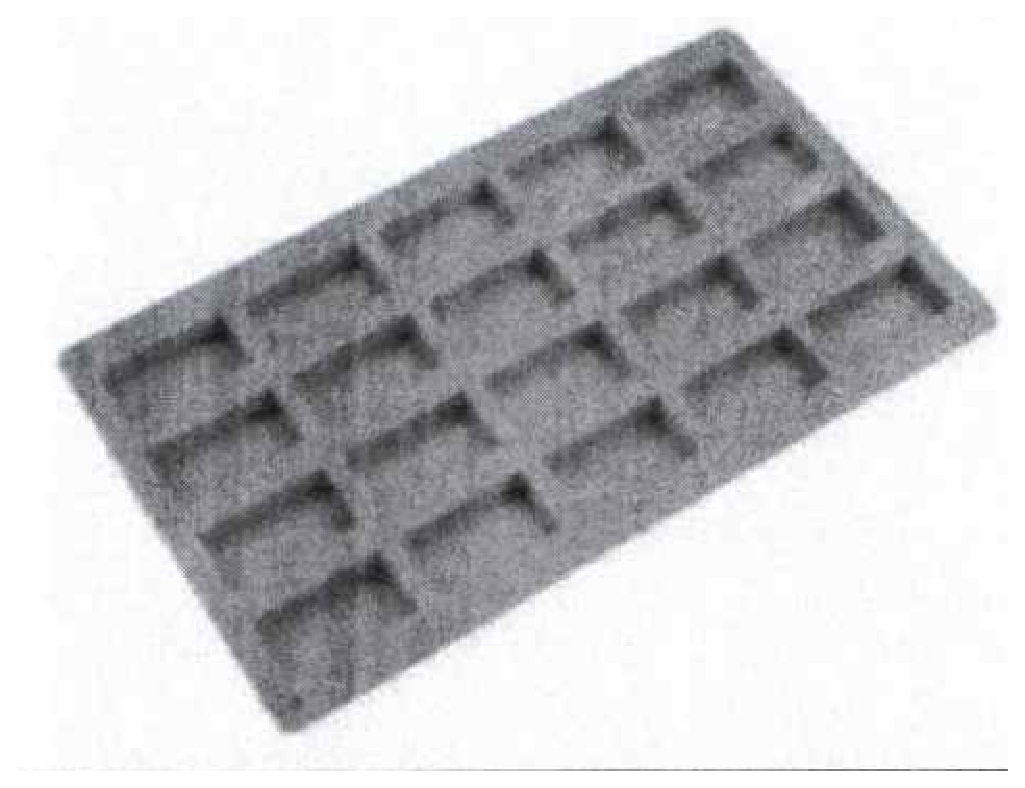
\includegraphics[width=6cm]{moule1}
\end{center}
\end{minipage}\hfill
\begin{minipage}{0.48\linewidth}
Chaque glaçon a la forme d'un pavé droit :
\begin{itemize}[label=$\bullet~~$]
\item de longueur 5 cm ;
\item de largeur 2,5 cm ;
\item de hauteur 1,5 cm.
\end{itemize}
\end{minipage}
\begin{enumerate}
\item On possède 12 moules à glaçons de ce type. Combien peut-on faire de glaçons en même temps ?
\item Montrer que le volume d'un glaçon est d'environ $19$~mL.\index{volume du pavé}
\item 5 litres d'eau sont-ils suffisants pour remplir ces 12 moules à glaçons ?
\end{enumerate}

\subsection*{Partie 2 : Le service}

\begin{minipage}{0.68\linewidth}
On souhaite servir le cocktail dans des verres cylindriques.

\begin{enumerate}[resume]
\item Montrer que le verre a un volume total d'environ $295$~mL.
\item Pour verser précisément $25$ cL de cocktail, on utilise des verres avec un repère indiquant une contenance de $25$~cL.
	\begin{enumerate}
		\item On a préparé $30$ litres de cocktail. Combien peut-on remplir de verres contenant $25$ cL de cocktail ?\index{volume du cylindre}
		\item En versant $25$ cL de cocktail dans le verre, à quelle hauteur $h$ du verre, le liquide arrive-t-il ?

Arrondir au dixième.
	\end{enumerate}
\end{enumerate}
\end{minipage}\hfill
\begin{minipage}{0.3\linewidth}
\psset{unit=1cm,arrowsize=2pt 3}
\begin{pspicture}(-2.7,0)(2.7,7.7)
\psellipse[linewidth=1.5pt](0,1.4)(1.05,0.3)
\psellipse[linewidth=1.5pt](0,1.45)(1.05,0.3)
\psellipse[linewidth=1.5pt](0,6.6)(1.05,0.3)
\psellipse[linewidth=1.5pt](0,6.65)(1.05,0.3)
\psline[linewidth=1.5pt](-1.05,1.4)(-1.05,6.65)
\psline[linewidth=1.5pt](1.05,1.4)(1.05,6.65)
\psellipse[linewidth=1.5pt,linestyle=dotted](0,5.7)(1.05,0.3)
\rput(0,7.6){Caractéristiques d'un verre}
\rput(1.8,6.3){Repère}\psline[linewidth=0.9pt]{->}(1.3,6.2)(0.6,5.44)
\psline[linewidth=0.9pt]{<->}(-1.5,1.4)(-1.5,6.6)\uput[l](-1.5,4){15 cm}
\psline[linewidth=0.9pt]{<->}(1.3,1.4)(1.3,5.6)\uput[r](1.3,3.5){$h$}
\psline[linewidth=0.9pt]{<->}(-1.05,0.8)(1.05,0.8)\uput[d](0,0.8){5 cm}
\end{pspicture}
\end{minipage}
%%%  fin Amérique du Sud 27 novembre 2025
\newpage
%%%  Nouvelle-Calédonie 11 décembre 2025
\phantomsection

\hypertarget{Caledoniedec}{}
\label{Caledoniedec}

\lfoot{\small{Nouvelle Calédonie}}
\rfoot{\small{11 décembre 2025}}
\setlength{\headheight}{13.59999pt}
\marginpar{\rotatebox{90}{\textbf{A. P{}. M. E. P{}.}}}
\pagestyle{fancy}
\thispagestyle{empty}
\begin{center}

{\Large \textbf{\decofourleft~Brevet des collèges Nouvelle Calédonie 11 décembre 2025~\decofourright}}

\bigskip

\textbf{Durée : 2 heures}

\medskip

\end{center}

\bigskip

\textbf{EXERCICE 1 : QCM \hfill 15 points}

\medskip

Cet exercice est un questionnaire à choix multiples (QCM).

Pour chaque question, une seule des trois réponses proposées est exacte.

Sur la copie, indiquer le numéro de la question et la réponse A, B ou C choisie. Aucune justification n'est demandée.

Aucun point ne sera enlevé en cas de mauvaise réponse.

\begin{center}
\begin{tabularx}{\linewidth}{|c|m{5.5cm}|*{3}{>{\centering \arraybackslash}X|}}\hline
\multicolumn{2}{|c|}{Questions}						&Réponse A	&Réponse B	&Réponse C\\ \hline
\textbf{1.}&Parmi les nombres suivants, lequel est premier ?	&719		&935		&687\\ \hline
\textbf{2.}&Quelle est l'aire de la figure ci-dessous ?

\begin{pspicture}(5.6,5)
\psset{arrowsize=2pt 3}
\def\bb{\psline(-0.05,-0.1)(-0.05,0.1)\psline(0.05,-0.1)(0.05,0.1)}
\pspolygon(0,4)(4.6,4)(4.6,0.7)(3.3,0.7)(3.3,2)(0,2)
\psframe(0,4)(0.2,3.8)\psframe(0,2)(0.2,2.2)\psframe(4.6,4)(4.4,3.8)
\psframe(4.6,0.7)(4.4,0.9)\psframe(3.3,0.7)(3.5,0.9)
\rput(3.95,0.7){\bb}\rput{90}(3.3,1.35){\bb}
\psline[linewidth=0.5pt]{<->}(0,4.2)(4.6,4.2)\uput[u](2.3,4.2){\small 7 cm}
\psline[linewidth=0.5pt]{<->}(4.8,4)(4.8,0.7)\uput[r](4.8,2.2){\small 5 cm}
\psline[linewidth=0.5pt]{<->}(4.6,0.5)(3.3,0.5)\uput[d](3.95,0.5){\small 2 cm}
\end{pspicture}&24 cm$^2$&140 cm$^2$&25 cm$^2$\\ 
\hline
\textbf{3.}& Une de ces fonctions est affine.\newline Laquelle ?&$f$ définie par $f(x) = 3 (x + 1 )$&$g$ définie par $g(x) = \dfrac{5}{x} + 1$\rule[-10pt]{0mm}{0pt}&$h$ définie par $h(x) =  x^2 + 1$\\ 
\hline
\textbf{4.}&La distance de Tontouta à Narita est égale à environ 6 980 km. Le vol Tontouta-Narita dure environ 9 heures. Quelle est la vitesse moyenne, arrondie à la centaine de km/h, de 
l'avion sur ce trajet ?&600 km/h&800 km/h&\np{1000} km/h\\
 \hline
\textbf{5.}&Dans un collège de 730 élèves, 60\,\% des élèves sont des filles.

Quel est le nombre de filles dans ce collège ?&438&60&670\\ 
\hline
\end{tabularx}
\end{center}

\newpage

\textbf{EXERCICE 2 : Cerf-volant \hfill 20 points}

\medskip

Thomas souhaite construire le cerf-volant représenté par la figure ci-dessous :

\begin{center}\begin{pspicture}(9.6,6)
%\psgrid
\pspolygon(2.3,5.6)(4.3,4.1)(2.3,0.7)(0.3,4.1)%ADBC
\psline(2.3,5.6)(2.3,0.7)%AB
\psline(4.3,4.1)(0.3,4.1)%CD
\psframe(2.3,4.1)(2.5,3.9)
\psline(1.25,4)(1.25,4.2)\psline(1.35,4)(1.35,4.2)
\psline(3.25,4)(3.25,4.2)\psline(3.35,4)(3.35,4.2)
\psarc(2.3,0.75){0.6}{58}{90}\rput(2.55,1.6){\small$30\degres$}
\uput[u](2.3,5.6){A} \uput[d](2.3,0.7){B} \uput[r](4.3,4.1){D} \uput[l](0.3,4.1){C} \uput[ur](2.3,4.1){E}
\rput(7.8,4.8){On donne :}
\rput(7.8,4.2){$\widehat{\text{DEB}} = 90\degres$\phantom{c}}
\rput(7.8,3.7){$\widehat{\text{EBD}} = 30\degres$\phantom{c}}
\rput(7.8,3.1){AB = 50 cm}
\rput(7.8,2.5){CD = 40 cm}
\rput(7.8,1.9){ED = EC\phantom{cm}}
\psframe(6.6,1.5)(8.8,5)
\end{pspicture}
\end{center}

\medskip

\begin{enumerate}
\item Calculer BE. On donnera une valeur arrondie au millimètre.

\textbf{Rédiger la réponse en faisant apparaitre les différentes étapes.}

\medskip

\begin{minipage}{0.7\linewidth}
Lorsque Thomas a essayé son cerf-volant, il s'est demandé à quelle altitude il volait.

Il a attaché sa corde à un piquet planté dans le sol (point S) puis est allé se placer (point T) parfaitement à la verticale
sous son cerf-volant (point H).

Il a alors mesuré certaines longueurs et a réalisé le schéma ci-contre.
\item Calculer HT, altitude à laquelle volait son cerf-volant. 

On donnera une valeur arrondie au mètre.

20,50 m
\textbf{Rédiger la réponse en faisant apparaitre les différentes étapes.}
\end{minipage}\hfill
\begin{minipage}{0.27\linewidth}
\psset{unit=1cm,arrowsize=2pt 3}
\begin{pspicture}(4.2,7.8)
\pspolygon(0.6,0.6)(2.8,0.6)(2.8,7.3)%STH
\psframe(2.8,0.6)(2.6,0.8)
\uput[dl](0.6,0.6){S} \uput[dr](2.8,0.6){T} \uput[u](2.8,7.3){H} 
\psline[linewidth=0.8pt]{<->}(0,0.8)(2.2,7.5)\uput[d](1.7,0.5){7,60 m}
\psline[linewidth=0.8pt]{<->}(0.6,0.4)(2.8,0.4)\rput{71.8}(1.5,4.3){20,50 m}
\end{pspicture}
\end{minipage}
\end{enumerate}

Il est conseillé de ne pas utiliser ce cerf-volant lorsque le vent dépasse $20$~km/h. La météo annonce un vent ne dépassant pas $15$ nœuds.

On donne 1 nœud $= 0,514$ m/s.

\begin{enumerate}[start=3]
\item Thomas peut-il faire voler son cerf-volant sans risque dans ces conditions ?

Justifier votre réponse.
\end{enumerate}

\newpage

\textbf{EXERCICE 3 Programmes de calcul \hfill 16 points}

\medskip

On considère les programmes de calcul suivants :

\begin{center}
%\renewcommand\arraystretch{1.2}
\begin{tabularx}{\linewidth}{|>{\centering \arraybackslash}X|c |>{\centering \arraybackslash}X|}\cline{1-1}\cline{3-3}
\textbf{PROGRAMME A}&&\textbf{PROGRAMME B}\\
\begin{itemize}[label=$\bullet~$]
\item Choisir un nombre
\item Ajouter 4
\item Multiplier par 3
\end{itemize}&&
\begin{itemize}[label=$\bullet~$]
\item Choisir un nombre 
\item Multiplier par 5
\item Soustraire 3
\item Soustraire le nombre de départ
\end{itemize}\\ \cline{1-1}\cline{3-3}
\end{tabularx}
\end{center}

\begin{enumerate}
\item Dans cette question, on choisit le nombre 2 pour tester les deux programmes.
	\begin{enumerate}
		\item Vérifier par le calcul qu'on obtient 18 avec le programme A.
		\item Vérifier par le calcul qu'on obtient 5 avec le programme B.
	\end{enumerate}
\item Soit $f$ la fonction associée au programme A, qui au nombre choisi $x$ fait correspondre
le résultat $f(x)$.
	\begin{enumerate}
		\item Justifier que $f(x) = 3x + 12$.
		\item Calculer l'antécédent de 27 par la fonction $f$.
	\end{enumerate}
\item Soit $g$ la fonction associée au programme B, qui au nombre choisi $x$ fait correspondre le résultat $g(x)$.
	\begin{enumerate}
		\item Donner l'expression de $g(x)$.
		\item Quel nombre faut-il choisir avec le programme B pour obtenir 2 comme résultat ?
		\end{enumerate}
\end{enumerate}
Hugo a choisi un nombre.

Il l'a testé avec les deux programmes et a trouvé le même résultat à chaque fois.

\begin{enumerate}[start=4]
\item Quel nombre a-t-il choisi ?
\end{enumerate}

\bigskip

\textbf{EXERCICE 4 : Jeu de hasard \hfill 13 points}

\medskip

Dans un jeu, les candidats doivent tirer une bille dans une boite et noter sa couleur, puis ils doivent ensuite lancer un dé de la couleur de la bille tirée et noter le résultat obtenu.

Les issues de cette expérience sont donc des couples du type (couleur~;~nombre).

Le matériel est le suivant :

\begin{description}
\item[ ] La boite contient des billes indiscernables au toucher :  {\red 15 rouges}, {\green 10 vertes} et  {\blue 5 bleues}.
\item[ ] Le dé rouge a 10 faces numérotées de 0 à 9. Le dé vert a 6 faces numérotées de 1 à 6.
\item[ ] Le dé bleu a 4 faces numérotées de 1 à 4.
\end{description}

\textbf{Pour gagner au jeu il faut obtenir 1 au lancé de dé.}

\begin{enumerate}
\item Quelle est la probabilité de tirer une bille bleue dans la boîte ?
\item Amandine a tiré une bille verte et Alexis a tiré une bille rouge.

Qui a le plus de chance de gagner à ce jeu ? Justifier.
\item Donner l'ensemble des issues possibles de ce jeu.

On notera \og R \fg pour rouge, \og V \fg pour vert et \og B \fg pour bleu.

Par exemple : l'issue (R~;~3) correspond à : \og la bille tirée est rouge et le résultat du lancer de dé est 3 \fg.
\end{enumerate}

\bigskip

\textbf{EXERCICE 5 : Géométrie \hfill 20 points}

\medskip

La figure ci-dessous n'est pas à l'échelle.

\begin{minipage}{0.4\linewidth}
\begin{tabular}{|l|}\hline
On donne :\\
~\\ 
AE = 6 cm \\
AD = 15 cm\\
BE = 4 cm\\
$\widehat{\text{BEA}} = \widehat{\text{CDA}} = 110\degres$\\
Les points A, B et C sont alignés\\
Les points A, E et D sont alignés\\ \hline
\end{tabular}
\end{minipage}\hfill
\begin{minipage}{0.65\linewidth}
\psset{unit=0.72cm,arrowsize=2pt 3}
\begin{pspicture}(11.6,7)
%\psgrid
\pspolygon(0.2,1)(9,1)(11.45,6.7)%ADC
\psline(3.6,1)(4.4,3.16)%EB
\uput[l](0.2,1){A} \uput[ul](4.9,3.4){B} \uput[ur](11.5,6.7){C} \uput[dr](9,1){D} \uput[dr](3.6,1){E}
\psline[linewidth=0.6pt]{<->}(0.2,0.8)(3.6,0.8)\uput[d](1.9,0.9){\small 6 cm}
\psline[linewidth=0.6pt]{<->}(0.2,0.3)(9,0.3)\uput[d](4.6,0.3){\small 15 cm}
\psarc(9,1){0.6}{70}{180}\uput[ul](8.8,1.3){$110\degres$}
\psarc(3.6,1){0.6}{70}{180}\uput[ul](3.4,1.3){$110\degres$}
\rput{70}(4.25,2.08){4 cm}
\end{pspicture}
\end{minipage}

\medskip

\begin{enumerate}
\item Prouver que les droites(BE) et (CD)sont parallèles. 
\item Calculer CD.

\textbf{Rédiger la réponse en faisant apparaitre les différentes étapes.}
\item L'aire du triangle ABE, arrondie au dixième, est égale à $11,3$cm$^2$.
En déduire l'aire du triangle ACD arrondie au dixième.
\item Construire cette figure en vraie grandeur sur l'annexe 1.
\end{enumerate}

\bigskip

\textbf{EXERCICE 6 : Scratch\hfill (16 points}

\medskip

\begin{enumerate}
\item 
Associer à chaque script ci-dessous la figure qui lui correspond.

\textbf{Sur la copie, indiquer le numéro du script et la figure correspondante.}

\begin{center}
\begin{tabularx}{\linewidth}{|*{3}{>{\centering \arraybackslash}X|}}\hline
\textbf{SCRIPT 1}&\textbf{SCRIPT 2}&\textbf{SCRIPT 3}\\ %
\begin{scratch}[scale=0.7]
\blockinit{quand \greenflag est cliqué}
\blockpen{stylo en position d'écriture}
\blockrepeat{répéter \ovalnum{3} fois}
{\blockmove{avancer de \ovalnum{100} pas}
\blockmove{tourner \turnright{} de \ovalnum{60} degrés}
}
\end{scratch}
&
\begin{scratch}[scale=0.7]
\blockinit{quand \greenflag est cliqué}
\blockpen{stylo en position d'écriture}
\blockrepeat{répéter \ovalnum{3} fois}
{\blockmove{avancer de \ovalnum{100} pas}
\blockmove{tourner \turnright{} de \ovalnum{90} degrés}
}
\end{scratch}
&
\begin{scratch}[scale=0.7]
\blockinit{quand \greenflag est cliqué}
\blockpen{stylo en position d'écriture}
\blockrepeat{répéter \ovalnum{3} fois}
{\blockmove{avancer de \ovalnum{100} pas}
\blockmove{tourner \turnright{} de \ovalnum{120} degrés}
}
\end{scratch}\\
&&\\
\hline
&&\\
FIGURE A&FIGURE B&FIGURE C\\ %\hline
\psset{unit=1cm}
\begin{pspicture}(1.5,1.5)
\psline(0,1)(1,1)(1,0)(0,0)
\end{pspicture}&
\psset{unit=1.414cm}
\begin{pspicture}(1.5,1.5)
\pspolygon(0,1)(1,1)(0.5,0.134)
\end{pspicture}
&\psset{unit=1cm}
\begin{pspicture}(0,-1)(1.5,1)
\psline(1;120)(1;60)(1;0)(1;-60)
\end{pspicture}\\ \hline
\end{tabularx}
\end{center}

\medskip

Le script ci-dessous commande la construction de la figure D.

\begin{center}
\begin{tabularx}{\linewidth}{p{4.5cm}p{2cm}X}
\begin{scratch}[scale=0.8]
\blockinit{quand \greenflag est cliqué}
\blockpen{stylo en position d'écriture}
\blockmove{avancer de \ovalnum{20} pas}
\blockmove{tourner \turnright{} de \ovalnum{90} degrés}
\blockmove{avancer de \ovalnum{40} pas}
\blockmove{tourner \turnright{} de \ovalnum{90} degrés}
\blockmove{avancer de \ovalnum{60} pas}
\blockmove{tourner \turnright{} de \ovalnum{90} degrés}
\blockmove{avancer de \ovalnum{80} pas}
\blockmove{tourner \turnright{} de \ovalnum{90} degrés}
\end{scratch}
&
\psset{unit=0.009cm}
\begin{pspicture}(-100,-100)(40,180)
\rput(-10,180){FIGURE D}
\psline(0,0)(40,0)(40,-100)(-100,-100)(-100,100)
\end{pspicture}
&
\psset{unit=0.9cm}
\begin{pspicture}(-3,-3)(4,4)
\psline[linewidth=1pt](0,0)(0.5,0)(0.5,-1)(-1,-1)(-1,1)(1.5,1)(1.50,-2)(-2,-2)(-2,2)(2.50,2)(2.50,-3)(-3,-3)(-3,3)(3.5,3)
\rput(.50,4){FIGURE E}
\end{pspicture}\\
\end{tabularx}
\end{center}

\item
Completer le script sur l'annexe 2 qui commande la construction de la figure E.
\end{enumerate}

\newpage

\begin{center}
\textbf{ANNEXE À RENDRE AVEC LA COPIE }
\end{center}
\bigskip

\textbf{Annexe 1 - Exercice 5 : Questions 4.}

Construire la figure en vraie grandeur

\vspace{6cm}

\begin{center}
\textbf{ANNEXE À RENDRE AVEC LA COPIE }
\end{center}

\bigskip

\textbf{Annexe 2 - Exercice 6 : Questions 2.}

\medskip

\begin{center}
\begin{scratch}
\blockinit{quand \greenflag est cliqué}
\blockvariable{mettre \selectmenu{longueur} à \ovalnum{~~~~~~}}
\blockpen{stylo en position d'écriture}
\blockrepeat{répéter \ovalnum{~~~~~~} fois}
{
\blockmove{avancer de \ovalcontrol{~~\ovalnum{~~~~~~~~~~~~~~~~}~~} pas}
\blockmove{tourner \turnright{} de \ovalnum{90} degrés}
\blockvariable{ajouter \ovalnum{~~~~~~} à \selectmenu{\ovalnum{~~~~~~~~~~~~~~}}}
}
\end{scratch}
\end{center}
%%%   fin Nouvelle-Calédonie 11 décembre 2025
\phantomsection
\hypertarget{Index}{}
\setlength{\columnsep}{1.5cm}
\printindex
\end{document}